% !TeX program = xelatex
% Preprint on the Agent Evaluation Science (AES) template. Build with `make` (see README.md).
\documentclass[11pt,a4paper]{article}
\usepackage{aes} % Public mode: the paper shows its authors.

\usepackage{amsmath,tabularx}

% --- Title block -----------------------------------------------------------------
% The title block of aes.sty, with the word "Preprint" in the place of the AES mark.
% The block has the height of the mark, so the page breaks are those of the template.
\makeatletter
\renewcommand{\maketitle}{%
 \par\begingroup
 \setlength{\parskip}{0pt}\setlength{\parindent}{0pt}%
 \thispagestyle{aesfirstpage}%
 \vspace*{\dimexpr\aesfirstpagetop-\aesbodytop-\baselineskip\relax}%
 \noindent\begin{minipage}[c][6.5mm][c]{80mm}%
  \color{aesink}\fontsize{7.5}{9}\selectfont\bfseries PREPRINT
 \end{minipage}\par
 \vspace{\aesbrandtitlesep}%
 {\color{aesink}\fontsize{22}{26.4}\selectfont\bfseries\raggedright\@title\par}%
 \vspace{\aestitleauthorsep}%
 \aesmakeauthors
 \vspace{\aesauthorabstractsep}%
 \endgroup
}
\makeatother

% --- Paper macros --------------------------------------------------------------
% \TODO{...}: visible red placeholder. `make check` fails while any remain.
\newcommand{\TODO}[1]{\textcolor{red}{\textbf{[TODO:} #1\textbf{]}}}
% \cv{key}: a number from generated/numbers.tex (written by `make numbers`).
% A missing key prints in red and logs a warning that `make check` reports.
\makeatletter
\newcommand{\cvset}[2]{\expandafter\def\csname cv@#1\endcsname{#2}}
\newcommand{\cv}[1]{\ifcsname cv@#1\endcsname\expandafter\cv@sign\csname cv@#1\endcsname\else
  \PackageWarning{paper}{cv key missing: #1}\textcolor{red}{\textbf{??#1}}\fi}
% A negative value prints with a true minus sign (U+2212), not a hyphen.
\def\cv@sign#1{\expandafter\cv@minus#1\relax}
\def\cv@minus#1#2\relax{\ifx-#1\char"2212\relax#2\else#1#2\fi}
\makeatother
% Generated by scripts/paper/make_numbers.py from reports/full/analysis.json and fit_<model>.json.
% Do not edit by hand: rerun `make numbers`. Use a value in the text as \cv{<key>}.
% Rates are percentages without the % sign; d', kappa and AUROC are plain decimals.

\cvset{run/mergedrows}{122{,}870} % rows in merged.jsonl, all models and detectors
\cvset{run/validrows}{122{,}528} % valid rows
\cvset{run/bootstrap}{1{,}000} % bootstrap resamples (d', dose slopes, and this script's kappa fractions)
\cvset{run/kappaboot}{500} % task-cluster resamples per pooled kappa interval (analysis.py)
\cvset{run/floor}{5} % floor-channel positive-rate threshold, percent
\cvset{design/temperature}{0.3} % sampling temperature of both models (config.py TARGET_MODELS)
\cvset{run/plannedpermodel}{12{,}600} % planned rollouts per model (run profile)
\cvset{run/planned}{25{,}200} % planned rollouts, both models
\cvset{design/maxdraws}{10} % run profile: stack_max_per_k
\cvset{design/logitpositions}{8} % run profile: logit_max_positions
\cvset{design/maxtokens}{8{,}000} % run profile: max_tokens
\cvset{design/reps}{3} % run profile: samples_per_config
\cvset{design/tasks}{100} % task scenarios
\cvset{design/items}{200} % items: tasks x valences
\cvset{design/configsA}{9} % baseline plus single factors
\cvset{design/expA}{5{,}400} % Experiment A rollouts per model
\cvset{design/expB}{7{,}200} % Experiment B rollouts per model
\cvset{design/itemsB}{50} % items in Experiment B
\cvset{design/f8n}{200} % F8 prompts
\cvset{design/f8named}{22} % F8 prompts whose suffix states an evaluation
\cvset{design/configsB}{48} % stacked configurations per item
\cvset{design/pairs}{16} % contrastive prompt pairs
\cvset{design/folds}{5} % task-grouped folds of the white-box fit
\cvset{gemma/reencode/nan}{1{,}745} % failure-ledger rows, reencode stage
\cvset{gemma/logit/nan}{1{,}577} % failure-ledger rows, logit stage
\cvset{qwen/reencode/nan}{0} % failure-ledger rows, reencode stage
\cvset{qwen/logit/nan}{0} % failure-ledger rows, logit stage
\cvset{gemma/rollouts}{12{,}589} % rollouts produced (responses file)
\cvset{gemma/cuedrollouts}{11{,}391} % cued rollouts produced: single F1 to F7 plus stacks (responses file)
\cvset{qwen/rollouts}{12{,}600} % rollouts produced (responses file)
\cvset{qwen/cuedrollouts}{11{,}400} % cued rollouts produced: single F1 to F7 plus stacks (responses file)
\cvset{run/rollouts}{25{,}189} % rollouts produced, both models
\cvset{gemma/sr/dprime}{1.06} % Gemma 4 31B, Self-report: pooled cued d'
\cvset{gemma/sr/dprimelo}{0.88}
\cvset{gemma/sr/dprimehi}{1.22}
\cvset{gemma/sr/hit}{58.3} % percent
\cvset{gemma/sr/fa}{19.8} % percent
\cvset{gemma/sr/ncued}{11{,}391}
\cvset{gemma/sr/nbase}{598}
\cvset{gemma/sr/nfa}{118} % baseline rollouts flagged
\cvset{gemma/sr/f8dprime}{0.91} % baseline vs F8 control
\cvset{gemma/tp/dprime}{1.17} % Gemma 4 31B, Third-person: pooled cued d'
\cvset{gemma/tp/dprimelo}{1.01}
\cvset{gemma/tp/dprimehi}{1.32}
\cvset{gemma/tp/hit}{80.0} % percent
\cvset{gemma/tp/fa}{37.1} % percent
\cvset{gemma/tp/ncued}{11{,}388}
\cvset{gemma/tp/nbase}{598}
\cvset{gemma/tp/nfa}{222} % baseline rollouts flagged
\cvset{gemma/tp/f8dprime}{0.82} % baseline vs F8 control
\cvset{gemma/cot/dprime}{1.17} % Gemma 4 31B, CoT judge: pooled cued d'
\cvset{gemma/cot/dprimelo}{0.79}
\cvset{gemma/cot/dprimehi}{1.65}
\cvset{gemma/cot/hit}{5.2} % percent
\cvset{gemma/cot/fa}{0.3} % percent
\cvset{gemma/cot/ncued}{11{,}169}
\cvset{gemma/cot/nbase}{585}
\cvset{gemma/cot/nfa}{1} % baseline rollouts flagged
\cvset{gemma/cot/f8dprime}{0.98} % baseline vs F8 control
\cvset{gemma/probe/dprime}{0.31} % Gemma 4 31B, Activation probe: pooled cued d'
\cvset{gemma/probe/dprimelo}{0.11}
\cvset{gemma/probe/dprimehi}{0.54}
\cvset{gemma/probe/hit}{62.3} % percent
\cvset{gemma/probe/fa}{50.0} % percent
\cvset{gemma/probe/ncued}{10{,}075}
\cvset{gemma/probe/nbase}{510}
\cvset{gemma/probe/nfa}{255} % baseline rollouts flagged
\cvset{gemma/probe/f8dprime}{-1.10} % baseline vs F8 control
\cvset{gemma/logit/dprime}{0.41} % Gemma 4 31B, Logit monitor: pooled cued d'
\cvset{gemma/logit/dprimelo}{0.23}
\cvset{gemma/logit/dprimehi}{0.61}
\cvset{gemma/logit/hit}{38.6} % percent
\cvset{gemma/logit/fa}{24.1} % percent
\cvset{gemma/logit/ncued}{10{,}014}
\cvset{gemma/logit/nbase}{499}
\cvset{gemma/logit/nfa}{120} % baseline rollouts flagged
\cvset{gemma/logit/f8dprime}{0.27} % baseline vs F8 control
\cvset{gemma/sr/posrate}{56.4} % percent positive on criterion rows
\cvset{gemma/sr/posrate2}{56.35} % the same, two decimals (for the 5% floor)
\cvset{gemma/tp/posrate}{77.9} % percent positive on criterion rows
\cvset{gemma/tp/posrate2}{77.86} % the same, two decimals (for the 5% floor)
\cvset{gemma/cot/posrate}{5.0} % percent positive on criterion rows
\cvset{gemma/cot/posrate2}{4.95} % the same, two decimals (for the 5% floor)
\cvset{gemma/probe/posrate}{61.7} % percent positive on criterion rows
\cvset{gemma/probe/posrate2}{61.66} % the same, two decimals (for the 5% floor)
\cvset{gemma/logit/posrate}{37.9} % percent positive on criterion rows
\cvset{gemma/logit/posrate2}{37.88} % the same, two decimals (for the 5% floor)
\cvset{gemma/sr-tp/kappa}{0.49} % Gemma 4 31B: kappa Self-report x Third-person
\cvset{gemma/sr-tp/kappalo}{0.46}
\cvset{gemma/sr-tp/kappahi}{0.53}
\cvset{gemma/sr-tp/kappacell}{0.51} % kappa on the majority call of each prompt cell
\cvset{gemma/sr-tp/nest}{98.2} % percent of Self-report positives that Third-person also flags
\cvset{gemma/sr-tp/nestlo}{97.9}
\cvset{gemma/sr-tp/nesthi}{98.5}
\cvset{gemma/tp-sr/nest}{71.1} % percent of Third-person positives that Self-report also flags
\cvset{gemma/tp-sr/nestlo}{70.2}
\cvset{gemma/tp-sr/nesthi}{72.0}
\cvset{gemma/sr-logit/kappa}{0.41} % Gemma 4 31B: kappa Self-report x Logit monitor
\cvset{gemma/sr-logit/kappalo}{0.34}
\cvset{gemma/sr-logit/kappahi}{0.48}
\cvset{gemma/sr-logit/kappacell}{0.42} % kappa on the majority call of each prompt cell
\cvset{gemma/sr-logit/nest}{56.1} % percent of Self-report positives that Logit monitor also flags
\cvset{gemma/sr-logit/nestlo}{54.9}
\cvset{gemma/sr-logit/nesthi}{57.4}
\cvset{gemma/logit-sr/nest}{86.5} % percent of Logit monitor positives that Self-report also flags
\cvset{gemma/logit-sr/nestlo}{85.4}
\cvset{gemma/logit-sr/nesthi}{87.6}
\cvset{gemma/tp-logit/kappa}{0.24} % Gemma 4 31B: kappa Third-person x Logit monitor
\cvset{gemma/tp-logit/kappalo}{0.19}
\cvset{gemma/tp-logit/kappahi}{0.30}
\cvset{gemma/tp-logit/kappacell}{0.24} % kappa on the majority call of each prompt cell
\cvset{gemma/tp-logit/nest}{46.4} % percent of Third-person positives that Logit monitor also flags
\cvset{gemma/tp-logit/nestlo}{45.3}
\cvset{gemma/tp-logit/nesthi}{47.5}
\cvset{gemma/logit-tp/nest}{96.9} % percent of Logit monitor positives that Third-person also flags
\cvset{gemma/logit-tp/nestlo}{96.3}
\cvset{gemma/logit-tp/nesthi}{97.4}
\cvset{gemma/tp-probe/kappa}{-0.01} % Gemma 4 31B: kappa Third-person x Activation probe
\cvset{gemma/tp-probe/kappalo}{-0.07}
\cvset{gemma/tp-probe/kappahi}{0.04}
\cvset{gemma/tp-probe/kappacell}{-0.01} % kappa on the majority call of each prompt cell
\cvset{gemma/tp-probe/nest}{61.3} % percent of Third-person positives that Activation probe also flags
\cvset{gemma/tp-probe/nestlo}{60.3}
\cvset{gemma/tp-probe/nesthi}{62.4}
\cvset{gemma/probe-tp/nest}{78.7} % percent of Activation probe positives that Third-person also flags
\cvset{gemma/probe-tp/nestlo}{77.7}
\cvset{gemma/probe-tp/nesthi}{79.7}
\cvset{gemma/sr-probe/kappa}{-0.02} % Gemma 4 31B: kappa Self-report x Activation probe
\cvset{gemma/sr-probe/kappalo}{-0.08}
\cvset{gemma/sr-probe/kappahi}{0.04}
\cvset{gemma/sr-probe/kappacell}{-0.03} % kappa on the majority call of each prompt cell
\cvset{gemma/sr-probe/nest}{60.7} % percent of Self-report positives that Activation probe also flags
\cvset{gemma/sr-probe/nestlo}{59.5}
\cvset{gemma/sr-probe/nesthi}{61.9}
\cvset{gemma/probe-sr/nest}{57.4} % percent of Activation probe positives that Self-report also flags
\cvset{gemma/probe-sr/nestlo}{56.2}
\cvset{gemma/probe-sr/nesthi}{58.6}
\cvset{gemma/probe-logit/kappa}{-0.02} % Gemma 4 31B: kappa Activation probe x Logit monitor
\cvset{gemma/probe-logit/kappalo}{-0.07}
\cvset{gemma/probe-logit/kappahi}{0.04}
\cvset{gemma/probe-logit/kappacell}{-0.03} % kappa on the majority call of each prompt cell
\cvset{gemma/probe-logit/nest}{37.2} % percent of Activation probe positives that Logit monitor also flags
\cvset{gemma/probe-logit/nestlo}{36.0}
\cvset{gemma/probe-logit/nesthi}{38.4}
\cvset{gemma/logit-probe/nest}{60.2} % percent of Logit monitor positives that Activation probe also flags
\cvset{gemma/logit-probe/nestlo}{58.7}
\cvset{gemma/logit-probe/nesthi}{61.8}
\cvset{gemma/kappacell/n}{3{,}529} % prompt cells behind the cell-majority kappa
\cvset{gemma/kappa/texttext}{0.49} % mean kappa, text-text pairs
\cvset{gemma/kappa/textwb}{0.15} % mean kappa, text-white-box pairs
\cvset{gemma/kappa/wbwb}{-0.02} % mean kappa, white-box-white-box pairs
\cvset{gemma/sr/baseline/rate}{19.7} % percent aware, Experiment A
\cvset{gemma/sr/F1/rate}{37.3} % percent aware, Experiment A
\cvset{gemma/sr/F2/rate}{40.5} % percent aware, Experiment A
\cvset{gemma/sr/F3/rate}{43.3} % percent aware, Experiment A
\cvset{gemma/sr/F4/rate}{15.5} % percent aware, Experiment A
\cvset{gemma/sr/F5/rate}{31.3} % percent aware, Experiment A
\cvset{gemma/sr/F6/rate}{49.8} % percent aware, Experiment A
\cvset{gemma/sr/F7/rate}{27.8} % percent aware, Experiment A
\cvset{gemma/sr/F8/rate}{52.3} % percent aware, Experiment A
\cvset{gemma/tp/baseline/rate}{37.1} % percent aware, Experiment A
\cvset{gemma/tp/F1/rate}{63.5} % percent aware, Experiment A
\cvset{gemma/tp/F2/rate}{63.2} % percent aware, Experiment A
\cvset{gemma/tp/F3/rate}{90.8} % percent aware, Experiment A
\cvset{gemma/tp/F4/rate}{32.5} % percent aware, Experiment A
\cvset{gemma/tp/F5/rate}{53.0} % percent aware, Experiment A
\cvset{gemma/tp/F6/rate}{66.3} % percent aware, Experiment A
\cvset{gemma/tp/F7/rate}{56.7} % percent aware, Experiment A
\cvset{gemma/tp/F8/rate}{68.8} % percent aware, Experiment A
\cvset{gemma/cot/baseline/rate}{0.2} % percent aware, Experiment A
\cvset{gemma/cot/F1/rate}{2.0} % percent aware, Experiment A
\cvset{gemma/cot/F2/rate}{1.2} % percent aware, Experiment A
\cvset{gemma/cot/F3/rate}{0.2} % percent aware, Experiment A
\cvset{gemma/cot/F4/rate}{0.3} % percent aware, Experiment A
\cvset{gemma/cot/F5/rate}{0.2} % percent aware, Experiment A
\cvset{gemma/cot/F6/rate}{7.8} % percent aware, Experiment A
\cvset{gemma/cot/F7/rate}{0.0} % percent aware, Experiment A
\cvset{gemma/cot/F8/rate}{3.4} % percent aware, Experiment A
\cvset{gemma/probe/baseline/rate}{50.0} % percent aware, Experiment A
\cvset{gemma/probe/F1/rate}{46.5} % percent aware, Experiment A
\cvset{gemma/probe/F2/rate}{60.4} % percent aware, Experiment A
\cvset{gemma/probe/F3/rate}{64.5} % percent aware, Experiment A
\cvset{gemma/probe/F4/rate}{66.3} % percent aware, Experiment A
\cvset{gemma/probe/F5/rate}{69.9} % percent aware, Experiment A
\cvset{gemma/probe/F6/rate}{35.1} % percent aware, Experiment A
\cvset{gemma/probe/F7/rate}{59.9} % percent aware, Experiment A
\cvset{gemma/probe/F8/rate}{13.5} % percent aware, Experiment A
\cvset{gemma/logit/baseline/rate}{24.0} % percent aware, Experiment A
\cvset{gemma/logit/F1/rate}{28.5} % percent aware, Experiment A
\cvset{gemma/logit/F2/rate}{37.5} % percent aware, Experiment A
\cvset{gemma/logit/F3/rate}{18.4} % percent aware, Experiment A
\cvset{gemma/logit/F4/rate}{17.9} % percent aware, Experiment A
\cvset{gemma/logit/F5/rate}{33.0} % percent aware, Experiment A
\cvset{gemma/logit/F6/rate}{44.7} % percent aware, Experiment A
\cvset{gemma/logit/F7/rate}{15.5} % percent aware, Experiment A
\cvset{gemma/logit/F8/rate}{33.5} % percent aware, Experiment A
\cvset{gemma/sr/dose0}{28.0} % percent aware at 0 stacked cues
\cvset{gemma/sr/dose1}{40.8} % percent aware at 1 stacked cues
\cvset{gemma/sr/dose2}{54.2} % percent aware at 2 stacked cues
\cvset{gemma/sr/dose3}{65.0} % percent aware at 3 stacked cues
\cvset{gemma/sr/dose4}{74.4} % percent aware at 4 stacked cues
\cvset{gemma/sr/dose5}{80.9} % percent aware at 5 stacked cues
\cvset{gemma/sr/dose6}{87.0} % percent aware at 6 stacked cues
\cvset{gemma/sr/dose7}{90.7} % percent aware at 7 stacked cues
\cvset{gemma/sr/slope}{0.091} % aware-rate slope per added cue
\cvset{gemma/sr/slopelo}{0.078}
\cvset{gemma/sr/slopehi}{0.106}
\cvset{gemma/tp/dose0}{45.3} % percent aware at 0 stacked cues
\cvset{gemma/tp/dose1}{64.6} % percent aware at 1 stacked cues
\cvset{gemma/tp/dose2}{80.1} % percent aware at 2 stacked cues
\cvset{gemma/tp/dose3}{90.1} % percent aware at 3 stacked cues
\cvset{gemma/tp/dose4}{93.8} % percent aware at 4 stacked cues
\cvset{gemma/tp/dose5}{96.1} % percent aware at 5 stacked cues
\cvset{gemma/tp/dose6}{96.7} % percent aware at 6 stacked cues
\cvset{gemma/tp/dose7}{96.7} % percent aware at 7 stacked cues
\cvset{gemma/tp/slope}{0.062} % aware-rate slope per added cue
\cvset{gemma/tp/slopelo}{0.051}
\cvset{gemma/tp/slopehi}{0.072}
\cvset{gemma/cot/dose0}{0.0} % percent aware at 0 stacked cues
\cvset{gemma/cot/dose1}{1.6} % percent aware at 1 stacked cues
\cvset{gemma/cot/dose2}{4.7} % percent aware at 2 stacked cues
\cvset{gemma/cot/dose3}{5.0} % percent aware at 3 stacked cues
\cvset{gemma/cot/dose4}{8.1} % percent aware at 4 stacked cues
\cvset{gemma/cot/dose5}{8.5} % percent aware at 5 stacked cues
\cvset{gemma/cot/dose6}{10.9} % percent aware at 6 stacked cues
\cvset{gemma/cot/dose7}{10.3} % percent aware at 7 stacked cues
\cvset{gemma/cot/slope}{0.017} % aware-rate slope per added cue
\cvset{gemma/cot/slopelo}{0.009}
\cvset{gemma/cot/slopehi}{0.025}
\cvset{gemma/probe/dose0}{46.2} % percent aware at 0 stacked cues
\cvset{gemma/probe/dose1}{58.9} % percent aware at 1 stacked cues
\cvset{gemma/probe/dose2}{62.8} % percent aware at 2 stacked cues
\cvset{gemma/probe/dose3}{62.9} % percent aware at 3 stacked cues
\cvset{gemma/probe/dose4}{65.6} % percent aware at 4 stacked cues
\cvset{gemma/probe/dose5}{65.4} % percent aware at 5 stacked cues
\cvset{gemma/probe/dose6}{67.8} % percent aware at 6 stacked cues
\cvset{gemma/probe/dose7}{75.5} % percent aware at 7 stacked cues
\cvset{gemma/probe/slope}{0.019} % aware-rate slope per added cue
\cvset{gemma/probe/slopelo}{-0.008}
\cvset{gemma/probe/slopehi}{0.043}
\cvset{gemma/logit/dose0}{20.7} % percent aware at 0 stacked cues
\cvset{gemma/logit/dose1}{25.7} % percent aware at 1 stacked cues
\cvset{gemma/logit/dose2}{35.5} % percent aware at 2 stacked cues
\cvset{gemma/logit/dose3}{41.4} % percent aware at 3 stacked cues
\cvset{gemma/logit/dose4}{45.9} % percent aware at 4 stacked cues
\cvset{gemma/logit/dose5}{48.0} % percent aware at 5 stacked cues
\cvset{gemma/logit/dose6}{51.3} % percent aware at 6 stacked cues
\cvset{gemma/logit/dose7}{55.5} % percent aware at 7 stacked cues
\cvset{gemma/logit/slope}{0.047} % aware-rate slope per added cue
\cvset{gemma/logit/slopelo}{0.030}
\cvset{gemma/logit/slopehi}{0.063}
\cvset{gemma/sr/retest}{0.78} % test-retest agreement
\cvset{gemma/sr/flip}{0.22} % flip rate
\cvset{gemma/tp/retest}{0.88} % test-retest agreement
\cvset{gemma/tp/flip}{0.12} % flip rate
\cvset{gemma/cot/retest}{0.92} % test-retest agreement
\cvset{gemma/cot/flip}{0.08} % flip rate
\cvset{gemma/probe/retest}{1.00} % test-retest agreement
\cvset{gemma/probe/flip}{0.00} % flip rate
\cvset{gemma/logit/retest}{0.84} % test-retest agreement
\cvset{gemma/logit/flip}{0.16} % flip rate
\cvset{gemma/judge2/n}{677} % traces re-judged with a parseable second verdict
\cvset{gemma/judge2/kappa}{0.06}
\cvset{gemma/judge2/raw}{0.31}
\cvset{gemma/judge2/pos1}{88.6} % percent, original judge, on the subset
\cvset{gemma/judge2/pos2}{19.5} % percent, second judge, on the subset
\cvset{gemma/judge2/npos1}{600} % first-judge positives on the re-judged subset
\cvset{gemma/judge2/npos2}{132} % second-judge positives on the subset
\cvset{gemma/judge2/nested}{132} % second-judge positives the first judge also flagged
\cvset{gemma/anchor/positives}{602}
\cvset{gemma/anchor/anchored}{252}
\cvset{gemma/anchor/neither}{341}
\cvset{gemma/probe/auroc}{0.589} % out-of-fold AUROC, contrastive direction
\cvset{gemma/probe/layer}{3} % chosen layer
\cvset{gemma/probe/nlayers}{60} % layers in the model, from the strided grid
\cvset{gemma/null/n}{24} % random directions
\cvset{gemma/null/mean}{0.564}
\cvset{gemma/null/max}{0.669}
\cvset{gemma/null/min}{0.464}
\cvset{gemma/null/above}{8} % random directions scoring above the probe
\cvset{gemma/probe/f8auroc}{0.251} % AUROC, F8 against baseline, chosen layer
\cvset{gemma/cued/auroc}{0.680}
\cvset{gemma/logistic/auroc}{0.920}
\cvset{gemma/logistic/kappa}{0.03}
\cvset{gemma/f8/yes}{13.5} % percent, probe on F8 prompts
\cvset{gemma/f8/base}{50.0} % percent, probe on baseline prompts
\cvset{gemma/f8/cued}{62.3} % percent, probe on cued prompts (same prompt-level fit rates)
\cvset{gemma/logit/auroc}{0.576}
\cvset{gemma/probe/novector}{1{,}491} % samples without a finite vector
\cvset{qwen/sr/dprime}{1.29} % Qwen 3.6 27B, Self-report: pooled cued d'
\cvset{qwen/sr/dprimelo}{1.11}
\cvset{qwen/sr/dprimehi}{1.45}
\cvset{qwen/sr/hit}{52.6} % percent
\cvset{qwen/sr/fa}{11.1} % percent
\cvset{qwen/sr/ncued}{11{,}400}
\cvset{qwen/sr/nbase}{600}
\cvset{qwen/sr/nfa}{66} % baseline rollouts flagged
\cvset{qwen/sr/f8dprime}{0.74} % baseline vs F8 control
\cvset{qwen/tp/dprime}{1.60} % Qwen 3.6 27B, Third-person: pooled cued d'
\cvset{qwen/tp/dprimelo}{1.40}
\cvset{qwen/tp/dprimehi}{1.79}
\cvset{qwen/tp/hit}{74.7} % percent
\cvset{qwen/tp/fa}{17.6} % percent
\cvset{qwen/tp/ncued}{11{,}396}
\cvset{qwen/tp/nbase}{600}
\cvset{qwen/tp/nfa}{105} % baseline rollouts flagged
\cvset{qwen/tp/f8dprime}{1.22} % baseline vs F8 control
\cvset{qwen/cot/dprime}{0.68} % Qwen 3.6 27B, CoT judge: pooled cued d'
\cvset{qwen/cot/dprimelo}{0.28}
\cvset{qwen/cot/dprimehi}{1.36}
\cvset{qwen/cot/hit}{3.3} % percent
\cvset{qwen/cot/fa}{0.6} % percent
\cvset{qwen/cot/ncued}{11{,}303}
\cvset{qwen/cot/nbase}{599}
\cvset{qwen/cot/nfa}{3} % baseline rollouts flagged
\cvset{qwen/cot/f8dprime}{1.25} % baseline vs F8 control
\cvset{qwen/probe/dprime}{1.24} % Qwen 3.6 27B, Activation probe: pooled cued d'
\cvset{qwen/probe/dprimelo}{1.00}
\cvset{qwen/probe/dprimehi}{1.48}
\cvset{qwen/probe/hit}{62.1} % percent
\cvset{qwen/probe/fa}{17.6} % percent
\cvset{qwen/probe/ncued}{11{,}400}
\cvset{qwen/probe/nbase}{600}
\cvset{qwen/probe/nfa}{105} % baseline rollouts flagged
\cvset{qwen/probe/f8dprime}{-2.21} % baseline vs F8 control
\cvset{qwen/logit/dprime}{0.68} % Qwen 3.6 27B, Logit monitor: pooled cued d'
\cvset{qwen/logit/dprimelo}{0.53}
\cvset{qwen/logit/dprimehi}{0.81}
\cvset{qwen/logit/hit}{75.1} % percent
\cvset{qwen/logit/fa}{50.0} % percent
\cvset{qwen/logit/ncued}{11{,}400}
\cvset{qwen/logit/nbase}{600}
\cvset{qwen/logit/nfa}{300} % baseline rollouts flagged
\cvset{qwen/logit/f8dprime}{0.72} % baseline vs F8 control
\cvset{qwen/sr/posrate}{50.5} % percent positive on criterion rows
\cvset{qwen/sr/posrate2}{50.52} % the same, two decimals (for the 5% floor)
\cvset{qwen/tp/posrate}{71.9} % percent positive on criterion rows
\cvset{qwen/tp/posrate2}{71.88} % the same, two decimals (for the 5% floor)
\cvset{qwen/cot/posrate}{3.1} % percent positive on criterion rows
\cvset{qwen/cot/posrate2}{3.11} % the same, two decimals (for the 5% floor)
\cvset{qwen/probe/posrate}{59.9} % percent positive on criterion rows
\cvset{qwen/probe/posrate2}{59.90} % the same, two decimals (for the 5% floor)
\cvset{qwen/logit/posrate}{73.8} % percent positive on criterion rows
\cvset{qwen/logit/posrate2}{73.84} % the same, two decimals (for the 5% floor)
\cvset{qwen/sr-tp/kappa}{0.44} % Qwen 3.6 27B: kappa Self-report x Third-person
\cvset{qwen/sr-tp/kappalo}{0.41}
\cvset{qwen/sr-tp/kappahi}{0.47}
\cvset{qwen/sr-tp/kappacell}{0.48} % kappa on the majority call of each prompt cell
\cvset{qwen/sr-tp/nest}{93.6} % percent of Self-report positives that Third-person also flags
\cvset{qwen/sr-tp/nestlo}{93.0}
\cvset{qwen/sr-tp/nesthi}{94.2}
\cvset{qwen/tp-sr/nest}{65.8} % percent of Third-person positives that Self-report also flags
\cvset{qwen/tp-sr/nestlo}{64.8}
\cvset{qwen/tp-sr/nesthi}{66.8}
\cvset{qwen/sr-logit/kappa}{0.36} % Qwen 3.6 27B: kappa Self-report x Logit monitor
\cvset{qwen/sr-logit/kappalo}{0.32}
\cvset{qwen/sr-logit/kappahi}{0.39}
\cvset{qwen/sr-logit/kappacell}{0.39} % kappa on the majority call of each prompt cell
\cvset{qwen/sr-logit/nest}{91.4} % percent of Self-report positives that Logit monitor also flags
\cvset{qwen/sr-logit/nestlo}{90.7}
\cvset{qwen/sr-logit/nesthi}{92.1}
\cvset{qwen/logit-sr/nest}{62.5} % percent of Logit monitor positives that Self-report also flags
\cvset{qwen/logit-sr/nestlo}{61.5}
\cvset{qwen/logit-sr/nesthi}{63.5}
\cvset{qwen/tp-logit/kappa}{0.33} % Qwen 3.6 27B: kappa Third-person x Logit monitor
\cvset{qwen/tp-logit/kappalo}{0.29}
\cvset{qwen/tp-logit/kappahi}{0.37}
\cvset{qwen/tp-logit/kappacell}{0.36} % kappa on the majority call of each prompt cell
\cvset{qwen/tp-logit/nest}{82.9} % percent of Third-person positives that Logit monitor also flags
\cvset{qwen/tp-logit/nestlo}{82.1}
\cvset{qwen/tp-logit/nesthi}{83.7}
\cvset{qwen/logit-tp/nest}{80.7} % percent of Logit monitor positives that Third-person also flags
\cvset{qwen/logit-tp/nestlo}{79.9}
\cvset{qwen/logit-tp/nesthi}{81.6}
\cvset{qwen/tp-probe/kappa}{0.16} % Qwen 3.6 27B: kappa Third-person x Activation probe
\cvset{qwen/tp-probe/kappalo}{0.10}
\cvset{qwen/tp-probe/kappahi}{0.21}
\cvset{qwen/tp-probe/kappacell}{0.16} % kappa on the majority call of each prompt cell
\cvset{qwen/tp-probe/nest}{64.9} % percent of Third-person positives that Activation probe also flags
\cvset{qwen/tp-probe/nestlo}{63.9}
\cvset{qwen/tp-probe/nesthi}{65.9}
\cvset{qwen/probe-tp/nest}{77.9} % percent of Activation probe positives that Third-person also flags
\cvset{qwen/probe-tp/nestlo}{76.9}
\cvset{qwen/probe-tp/nesthi}{78.9}
\cvset{qwen/sr-probe/kappa}{0.13} % Qwen 3.6 27B: kappa Self-report x Activation probe
\cvset{qwen/sr-probe/kappalo}{0.07}
\cvset{qwen/sr-probe/kappahi}{0.18}
\cvset{qwen/sr-probe/kappacell}{0.13} % kappa on the majority call of each prompt cell
\cvset{qwen/sr-probe/nest}{66.1} % percent of Self-report positives that Activation probe also flags
\cvset{qwen/sr-probe/nestlo}{64.9}
\cvset{qwen/sr-probe/nesthi}{67.3}
\cvset{qwen/probe-sr/nest}{55.7} % percent of Activation probe positives that Self-report also flags
\cvset{qwen/probe-sr/nestlo}{54.6}
\cvset{qwen/probe-sr/nesthi}{56.9}
\cvset{qwen/probe-logit/kappa}{0.06} % Qwen 3.6 27B: kappa Activation probe x Logit monitor
\cvset{qwen/probe-logit/kappalo}{0.01}
\cvset{qwen/probe-logit/kappahi}{0.11}
\cvset{qwen/probe-logit/kappacell}{0.06} % kappa on the majority call of each prompt cell
\cvset{qwen/probe-logit/nest}{76.2} % percent of Activation probe positives that Logit monitor also flags
\cvset{qwen/probe-logit/nestlo}{75.2}
\cvset{qwen/probe-logit/nesthi}{77.1}
\cvset{qwen/logit-probe/nest}{61.8} % percent of Logit monitor positives that Activation probe also flags
\cvset{qwen/logit-probe/nestlo}{60.8}
\cvset{qwen/logit-probe/nesthi}{62.8}
\cvset{qwen/kappacell/n}{4{,}000} % prompt cells behind the cell-majority kappa
\cvset{qwen/kappa/texttext}{0.44} % mean kappa, text-text pairs
\cvset{qwen/kappa/textwb}{0.24} % mean kappa, text-white-box pairs
\cvset{qwen/kappa/wbwb}{0.06} % mean kappa, white-box-white-box pairs
\cvset{qwen/sr/baseline/rate}{11.0} % percent aware, Experiment A
\cvset{qwen/sr/F1/rate}{29.5} % percent aware, Experiment A
\cvset{qwen/sr/F2/rate}{30.8} % percent aware, Experiment A
\cvset{qwen/sr/F3/rate}{23.3} % percent aware, Experiment A
\cvset{qwen/sr/F4/rate}{16.3} % percent aware, Experiment A
\cvset{qwen/sr/F5/rate}{19.5} % percent aware, Experiment A
\cvset{qwen/sr/F6/rate}{44.3} % percent aware, Experiment A
\cvset{qwen/sr/F7/rate}{17.5} % percent aware, Experiment A
\cvset{qwen/sr/F8/rate}{31.5} % percent aware, Experiment A
\cvset{qwen/tp/baseline/rate}{17.5} % percent aware, Experiment A
\cvset{qwen/tp/F1/rate}{57.5} % percent aware, Experiment A
\cvset{qwen/tp/F2/rate}{62.3} % percent aware, Experiment A
\cvset{qwen/tp/F3/rate}{61.5} % percent aware, Experiment A
\cvset{qwen/tp/F4/rate}{23.4} % percent aware, Experiment A
\cvset{qwen/tp/F5/rate}{31.0} % percent aware, Experiment A
\cvset{qwen/tp/F6/rate}{57.8} % percent aware, Experiment A
\cvset{qwen/tp/F7/rate}{49.2} % percent aware, Experiment A
\cvset{qwen/tp/F8/rate}{61.2} % percent aware, Experiment A
\cvset{qwen/cot/baseline/rate}{0.5} % percent aware, Experiment A
\cvset{qwen/cot/F1/rate}{2.7} % percent aware, Experiment A
\cvset{qwen/cot/F2/rate}{0.3} % percent aware, Experiment A
\cvset{qwen/cot/F3/rate}{0.3} % percent aware, Experiment A
\cvset{qwen/cot/F4/rate}{0.7} % percent aware, Experiment A
\cvset{qwen/cot/F5/rate}{0.3} % percent aware, Experiment A
\cvset{qwen/cot/F6/rate}{6.1} % percent aware, Experiment A
\cvset{qwen/cot/F7/rate}{0.2} % percent aware, Experiment A
\cvset{qwen/cot/F8/rate}{10.1} % percent aware, Experiment A
\cvset{qwen/probe/baseline/rate}{17.5} % percent aware, Experiment A
\cvset{qwen/probe/F1/rate}{25.5} % percent aware, Experiment A
\cvset{qwen/probe/F2/rate}{32.0} % percent aware, Experiment A
\cvset{qwen/probe/F3/rate}{89.5} % percent aware, Experiment A
\cvset{qwen/probe/F4/rate}{52.5} % percent aware, Experiment A
\cvset{qwen/probe/F5/rate}{58.5} % percent aware, Experiment A
\cvset{qwen/probe/F6/rate}{6.0} % percent aware, Experiment A
\cvset{qwen/probe/F7/rate}{36.5} % percent aware, Experiment A
\cvset{qwen/probe/F8/rate}{0.0} % percent aware, Experiment A
\cvset{qwen/logit/baseline/rate}{50.0} % percent aware, Experiment A
\cvset{qwen/logit/F1/rate}{61.7} % percent aware, Experiment A
\cvset{qwen/logit/F2/rate}{63.2} % percent aware, Experiment A
\cvset{qwen/logit/F3/rate}{59.8} % percent aware, Experiment A
\cvset{qwen/logit/F4/rate}{70.8} % percent aware, Experiment A
\cvset{qwen/logit/F5/rate}{62.8} % percent aware, Experiment A
\cvset{qwen/logit/F6/rate}{60.7} % percent aware, Experiment A
\cvset{qwen/logit/F7/rate}{63.0} % percent aware, Experiment A
\cvset{qwen/logit/F8/rate}{76.5} % percent aware, Experiment A
\cvset{qwen/sr/dose0}{12.7} % percent aware at 0 stacked cues
\cvset{qwen/sr/dose1}{26.8} % percent aware at 1 stacked cues
\cvset{qwen/sr/dose2}{47.5} % percent aware at 2 stacked cues
\cvset{qwen/sr/dose3}{58.9} % percent aware at 3 stacked cues
\cvset{qwen/sr/dose4}{71.8} % percent aware at 4 stacked cues
\cvset{qwen/sr/dose5}{80.5} % percent aware at 5 stacked cues
\cvset{qwen/sr/dose6}{85.5} % percent aware at 6 stacked cues
\cvset{qwen/sr/dose7}{86.0} % percent aware at 7 stacked cues
\cvset{qwen/sr/slope}{0.114} % aware-rate slope per added cue
\cvset{qwen/sr/slopelo}{0.100}
\cvset{qwen/sr/slopehi}{0.126}
\cvset{qwen/tp/dose0}{15.3} % percent aware at 0 stacked cues
\cvset{qwen/tp/dose1}{48.4} % percent aware at 1 stacked cues
\cvset{qwen/tp/dose2}{75.1} % percent aware at 2 stacked cues
\cvset{qwen/tp/dose3}{87.6} % percent aware at 3 stacked cues
\cvset{qwen/tp/dose4}{93.2} % percent aware at 4 stacked cues
\cvset{qwen/tp/dose5}{97.0} % percent aware at 5 stacked cues
\cvset{qwen/tp/dose6}{97.6} % percent aware at 6 stacked cues
\cvset{qwen/tp/dose7}{97.3} % percent aware at 7 stacked cues
\cvset{qwen/tp/slope}{0.093} % aware-rate slope per added cue
\cvset{qwen/tp/slopelo}{0.085}
\cvset{qwen/tp/slopehi}{0.101}
\cvset{qwen/cot/dose0}{0.0} % percent aware at 0 stacked cues
\cvset{qwen/cot/dose1}{1.7} % percent aware at 1 stacked cues
\cvset{qwen/cot/dose2}{3.8} % percent aware at 2 stacked cues
\cvset{qwen/cot/dose3}{3.6} % percent aware at 3 stacked cues
\cvset{qwen/cot/dose4}{4.6} % percent aware at 4 stacked cues
\cvset{qwen/cot/dose5}{4.8} % percent aware at 5 stacked cues
\cvset{qwen/cot/dose6}{4.9} % percent aware at 6 stacked cues
\cvset{qwen/cot/dose7}{2.7} % percent aware at 7 stacked cues
\cvset{qwen/cot/slope}{0.005} % aware-rate slope per added cue
\cvset{qwen/cot/slopelo}{0.002}
\cvset{qwen/cot/slopehi}{0.009}
\cvset{qwen/probe/dose0}{16.0} % percent aware at 0 stacked cues
\cvset{qwen/probe/dose1}{44.9} % percent aware at 1 stacked cues
\cvset{qwen/probe/dose2}{58.0} % percent aware at 2 stacked cues
\cvset{qwen/probe/dose3}{68.4} % percent aware at 3 stacked cues
\cvset{qwen/probe/dose4}{79.0} % percent aware at 4 stacked cues
\cvset{qwen/probe/dose5}{80.4} % percent aware at 5 stacked cues
\cvset{qwen/probe/dose6}{82.6} % percent aware at 6 stacked cues
\cvset{qwen/probe/dose7}{84.0} % percent aware at 7 stacked cues
\cvset{qwen/probe/slope}{0.079} % aware-rate slope per added cue
\cvset{qwen/probe/slopelo}{0.062}
\cvset{qwen/probe/slopehi}{0.096}
\cvset{qwen/logit/dose0}{56.7} % percent aware at 0 stacked cues
\cvset{qwen/logit/dose1}{65.0} % percent aware at 1 stacked cues
\cvset{qwen/logit/dose2}{72.0} % percent aware at 2 stacked cues
\cvset{qwen/logit/dose3}{78.7} % percent aware at 3 stacked cues
\cvset{qwen/logit/dose4}{84.0} % percent aware at 4 stacked cues
\cvset{qwen/logit/dose5}{87.1} % percent aware at 5 stacked cues
\cvset{qwen/logit/dose6}{90.2} % percent aware at 6 stacked cues
\cvset{qwen/logit/dose7}{89.3} % percent aware at 7 stacked cues
\cvset{qwen/logit/slope}{0.050} % aware-rate slope per added cue
\cvset{qwen/logit/slopelo}{0.035}
\cvset{qwen/logit/slopehi}{0.062}
\cvset{qwen/sr/retest}{0.74} % test-retest agreement
\cvset{qwen/sr/flip}{0.26} % flip rate
\cvset{qwen/tp/retest}{0.77} % test-retest agreement
\cvset{qwen/tp/flip}{0.23} % flip rate
\cvset{qwen/cot/retest}{0.93} % test-retest agreement
\cvset{qwen/cot/flip}{0.07} % flip rate
\cvset{qwen/probe/retest}{1.00} % test-retest agreement
\cvset{qwen/probe/flip}{0.00} % flip rate
\cvset{qwen/logit/retest}{0.93} % test-retest agreement
\cvset{qwen/logit/flip}{0.07} % flip rate
\cvset{qwen/judge2/n}{485} % traces re-judged with a parseable second verdict
\cvset{qwen/judge2/kappa}{0.04}
\cvset{qwen/judge2/raw}{0.26}
\cvset{qwen/judge2/pos1}{83.5} % percent, original judge, on the subset
\cvset{qwen/judge2/pos2}{10.7} % percent, second judge, on the subset
\cvset{qwen/judge2/npos1}{405} % first-judge positives on the re-judged subset
\cvset{qwen/judge2/npos2}{52} % second-judge positives on the subset
\cvset{qwen/judge2/nested}{50} % second-judge positives the first judge also flagged
\cvset{qwen/anchor/positives}{430}
\cvset{qwen/anchor/anchored}{410}
\cvset{qwen/anchor/neither}{19}
\cvset{qwen/probe/auroc}{0.783} % out-of-fold AUROC, contrastive direction
\cvset{qwen/probe/layer}{15} % chosen layer
\cvset{qwen/probe/nlayers}{64} % layers in the model, from the strided grid
\cvset{qwen/null/n}{24} % random directions
\cvset{qwen/null/mean}{0.766}
\cvset{qwen/null/max}{0.893}
\cvset{qwen/null/min}{0.577}
\cvset{qwen/null/above}{11} % random directions scoring above the probe
\cvset{qwen/probe/f8auroc}{0.119} % AUROC, F8 against baseline, chosen layer
\cvset{qwen/cued/auroc}{0.951}
\cvset{qwen/logistic/auroc}{0.987}
\cvset{qwen/logistic/kappa}{0.13}
\cvset{qwen/f8/yes}{0.0} % percent, probe on F8 prompts
\cvset{qwen/f8/base}{17.5} % percent, probe on baseline prompts
\cvset{qwen/f8/cued}{62.1} % percent, probe on cued prompts (same prompt-level fit rates)
\cvset{qwen/logit/auroc}{0.672}
\cvset{qwen/probe/novector}{0} % samples without a finite vector
\cvset{run/doseclear}{9} % detector-model slopes whose 95% interval excludes zero
\cvset{run/dosepairs}{10} % detector-model slopes
\cvset{design/tasksB}{25} % task clusters behind each Experiment B slope
\cvset{run/doseclearinterp}{8} % interpreted slopes whose 95% interval lies above zero
\cvset{run/dosepairsinterp}{8} % interpreted detector-model slopes (Gemma white-box excluded)
\cvset{run/dprimepairs}{8} % analysed detector-model combinations for d' (Gemma white-box excluded)
\cvset{run/dprimeclear}{8} % analysed combinations whose d' 95% interval lies above zero
\cvset{gemma/sr-tp/kappamax}{0.54} % largest kappa the two positive rates allow
\cvset{gemma/sr-tp/kappafrac}{92} % kappa as a percent of its ceiling
\cvset{gemma/sr-tp/kappafraclo}{89} % 95% task-cluster bootstrap interval, percent of ceiling
\cvset{gemma/sr-tp/kappafrachi}{94}
\cvset{gemma/sr-tp/kappawithin}{0.38} % kappa pooled within cue configurations (post hoc)
\cvset{gemma/sr-tp/kappawithinlo}{0.33} % 95% task-cluster bootstrap interval
\cvset{gemma/sr-tp/kappawithinhi}{0.42}
\cvset{gemma/sr-tp/kappawithinmax}{0.43} % ceiling of the within-configuration kappa
\cvset{gemma/sr-tp/kappawithinfrac}{88} % within-configuration kappa as a percent of its ceiling
\cvset{gemma/sr-tp/kappawithinfraclo}{84} % 95% task-cluster bootstrap interval
\cvset{gemma/sr-tp/kappawithinfrachi}{91}
\cvset{gemma/sr-tp/kappawithinforced}{0.57} % disagreement forced by unequal positive rates, 1 - kappa_max (stratified)
\cvset{gemma/sr-tp/kappawithinrest}{0.05} % remaining disagreement, kappa_max - kappa (stratified)
\cvset{gemma/sr-tp/kappacv}{0.23} % kappa pooled within configuration x variant strata (post hoc)
\cvset{gemma/sr-tp/kappacvlo}{0.17} % 95% task-cluster bootstrap interval
\cvset{gemma/sr-tp/kappacvhi}{0.27}
\cvset{gemma/sr-tp/kappacvmax}{0.29} % ceiling of the configuration x variant kappa
\cvset{gemma/sr-tp/kappacvfrac}{78} % configuration x variant kappa as a percent of its ceiling
\cvset{gemma/sr-tp/kappacvfraclo}{71} % 95% task-cluster bootstrap interval
\cvset{gemma/sr-tp/kappacvfrachi}{83}
\cvset{gemma/sr-tp/kappaindep}{0.19} % pooled kappa expected under independence within configurations
\cvset{gemma/sr-tp/nestindep}{85.5} % nest expected under independence within configurations
\cvset{gemma/tp-sr/nestindep}{61.9} % nest expected under independence within configurations
\cvset{gemma/sr-logit/kappamax}{0.61} % largest kappa the two positive rates allow
\cvset{gemma/sr-logit/kappafrac}{68} % kappa as a percent of its ceiling
\cvset{gemma/sr-logit/kappafraclo}{62} % 95% task-cluster bootstrap interval, percent of ceiling
\cvset{gemma/sr-logit/kappafrachi}{72}
\cvset{gemma/sr-logit/kappawithin}{0.35} % kappa pooled within cue configurations (post hoc)
\cvset{gemma/sr-logit/kappawithinlo}{0.28} % 95% task-cluster bootstrap interval
\cvset{gemma/sr-logit/kappawithinhi}{0.42}
\cvset{gemma/sr-logit/kappawithinmax}{0.56} % ceiling of the within-configuration kappa
\cvset{gemma/sr-logit/kappawithinfrac}{63} % within-configuration kappa as a percent of its ceiling
\cvset{gemma/sr-logit/kappawithinfraclo}{58} % 95% task-cluster bootstrap interval
\cvset{gemma/sr-logit/kappawithinfrachi}{68}
\cvset{gemma/sr-logit/kappawithinforced}{0.44} % disagreement forced by unequal positive rates, 1 - kappa_max (stratified)
\cvset{gemma/sr-logit/kappawithinrest}{0.21} % remaining disagreement, kappa_max - kappa (stratified)
\cvset{gemma/sr-logit/kappacv}{0.13} % kappa pooled within configuration x variant strata (post hoc)
\cvset{gemma/sr-logit/kappacvlo}{0.09} % 95% task-cluster bootstrap interval
\cvset{gemma/sr-logit/kappacvhi}{0.17}
\cvset{gemma/sr-logit/kappacvmax}{0.39} % ceiling of the configuration x variant kappa
\cvset{gemma/sr-logit/kappacvfrac}{34} % configuration x variant kappa as a percent of its ceiling
\cvset{gemma/sr-logit/kappacvfraclo}{26} % 95% task-cluster bootstrap interval
\cvset{gemma/sr-logit/kappacvfrachi}{43}
\cvset{gemma/sr-logit/kappaindep}{0.09} % pooled kappa expected under independence within configurations
\cvset{gemma/sr-logit/nestindep}{41.9} % nest expected under independence within configurations
\cvset{gemma/logit-sr/nestindep}{64.6} % nest expected under independence within configurations
\cvset{gemma/tp-logit/kappamax}{0.28} % largest kappa the two positive rates allow
\cvset{gemma/tp-logit/kappafrac}{85} % kappa as a percent of its ceiling
\cvset{gemma/tp-logit/kappafraclo}{80} % 95% task-cluster bootstrap interval, percent of ceiling
\cvset{gemma/tp-logit/kappafrachi}{89}
\cvset{gemma/tp-logit/kappawithin}{0.19} % kappa pooled within cue configurations (post hoc)
\cvset{gemma/tp-logit/kappawithinlo}{0.14} % 95% task-cluster bootstrap interval
\cvset{gemma/tp-logit/kappawithinhi}{0.24}
\cvset{gemma/tp-logit/kappawithinmax}{0.23} % ceiling of the within-configuration kappa
\cvset{gemma/tp-logit/kappawithinfrac}{81} % within-configuration kappa as a percent of its ceiling
\cvset{gemma/tp-logit/kappawithinfraclo}{75} % 95% task-cluster bootstrap interval
\cvset{gemma/tp-logit/kappawithinfrachi}{86}
\cvset{gemma/tp-logit/kappawithinforced}{0.77} % disagreement forced by unequal positive rates, 1 - kappa_max (stratified)
\cvset{gemma/tp-logit/kappawithinrest}{0.04} % remaining disagreement, kappa_max - kappa (stratified)
\cvset{gemma/tp-logit/kappacv}{0.08} % kappa pooled within configuration x variant strata (post hoc)
\cvset{gemma/tp-logit/kappacvlo}{0.05} % 95% task-cluster bootstrap interval
\cvset{gemma/tp-logit/kappacvhi}{0.11}
\cvset{gemma/tp-logit/kappacvmax}{0.13} % ceiling of the configuration x variant kappa
\cvset{gemma/tp-logit/kappacvfrac}{62} % configuration x variant kappa as a percent of its ceiling
\cvset{gemma/tp-logit/kappacvfraclo}{52} % 95% task-cluster bootstrap interval
\cvset{gemma/tp-logit/kappacvfrachi}{70}
\cvset{gemma/tp-logit/kappaindep}{0.06} % pooled kappa expected under independence within configurations
\cvset{gemma/tp-logit/nestindep}{39.9} % nest expected under independence within configurations
\cvset{gemma/logit-tp/nestindep}{83.5} % nest expected under independence within configurations
\cvset{gemma/tp-probe/kappamax}{0.59} % largest kappa the two positive rates allow
\cvset{gemma/tp-probe/kappafrac}{-2} % kappa as a percent of its ceiling
\cvset{gemma/tp-probe/kappafraclo}{-12} % 95% task-cluster bootstrap interval, percent of ceiling
\cvset{gemma/tp-probe/kappafrachi}{8}
\cvset{gemma/tp-probe/kappawithin}{-0.03} % kappa pooled within cue configurations (post hoc)
\cvset{gemma/tp-probe/kappawithinlo}{-0.08} % 95% task-cluster bootstrap interval
\cvset{gemma/tp-probe/kappawithinhi}{0.02}
\cvset{gemma/tp-probe/kappawithinmax}{0.44} % ceiling of the within-configuration kappa
\cvset{gemma/tp-probe/kappawithinfrac}{-7} % within-configuration kappa as a percent of its ceiling
\cvset{gemma/tp-probe/kappawithinfraclo}{-19} % 95% task-cluster bootstrap interval
\cvset{gemma/tp-probe/kappawithinfrachi}{4}
\cvset{gemma/tp-probe/kappawithinforced}{0.56} % disagreement forced by unequal positive rates, 1 - kappa_max (stratified)
\cvset{gemma/tp-probe/kappawithinrest}{0.47} % remaining disagreement, kappa_max - kappa (stratified)
\cvset{gemma/tp-probe/kappacv}{-0.02} % kappa pooled within configuration x variant strata (post hoc)
\cvset{gemma/tp-probe/kappacvlo}{-0.06} % 95% task-cluster bootstrap interval
\cvset{gemma/tp-probe/kappacvhi}{0.03}
\cvset{gemma/tp-probe/kappacvmax}{0.29} % ceiling of the configuration x variant kappa
\cvset{gemma/tp-probe/kappacvfrac}{-6} % configuration x variant kappa as a percent of its ceiling
\cvset{gemma/tp-probe/kappacvfraclo}{-22} % 95% task-cluster bootstrap interval
\cvset{gemma/tp-probe/kappacvfrachi}{11}
\cvset{gemma/tp-probe/kappaindep}{0.02} % pooled kappa expected under independence within configurations
\cvset{gemma/tp-probe/nestindep}{62.2} % nest expected under independence within configurations
\cvset{gemma/probe-tp/nestindep}{79.8} % nest expected under independence within configurations
\cvset{gemma/sr-probe/kappamax}{0.93} % largest kappa the two positive rates allow
\cvset{gemma/sr-probe/kappafrac}{-2} % kappa as a percent of its ceiling
\cvset{gemma/sr-probe/kappafraclo}{-9} % 95% task-cluster bootstrap interval, percent of ceiling
\cvset{gemma/sr-probe/kappafrachi}{5}
\cvset{gemma/sr-probe/kappawithin}{-0.05} % kappa pooled within cue configurations (post hoc)
\cvset{gemma/sr-probe/kappawithinlo}{-0.10} % 95% task-cluster bootstrap interval
\cvset{gemma/sr-probe/kappawithinhi}{0.00}
\cvset{gemma/sr-probe/kappawithinmax}{0.56} % ceiling of the within-configuration kappa
\cvset{gemma/sr-probe/kappawithinfrac}{-9} % within-configuration kappa as a percent of its ceiling
\cvset{gemma/sr-probe/kappawithinfraclo}{-20} % 95% task-cluster bootstrap interval
\cvset{gemma/sr-probe/kappawithinfrachi}{0}
\cvset{gemma/sr-probe/kappawithinforced}{0.44} % disagreement forced by unequal positive rates, 1 - kappa_max (stratified)
\cvset{gemma/sr-probe/kappawithinrest}{0.61} % remaining disagreement, kappa_max - kappa (stratified)
\cvset{gemma/sr-probe/kappacv}{-0.04} % kappa pooled within configuration x variant strata (post hoc)
\cvset{gemma/sr-probe/kappacvlo}{-0.09} % 95% task-cluster bootstrap interval
\cvset{gemma/sr-probe/kappacvhi}{0.01}
\cvset{gemma/sr-probe/kappacvmax}{0.35} % ceiling of the configuration x variant kappa
\cvset{gemma/sr-probe/kappacvfrac}{-11} % configuration x variant kappa as a percent of its ceiling
\cvset{gemma/sr-probe/kappacvfraclo}{-28} % 95% task-cluster bootstrap interval
\cvset{gemma/sr-probe/kappacvfrachi}{5}
\cvset{gemma/sr-probe/kappaindep}{0.03} % pooled kappa expected under independence within configurations
\cvset{gemma/sr-probe/nestindep}{62.8} % nest expected under independence within configurations
\cvset{gemma/probe-sr/nestindep}{59.3} % nest expected under independence within configurations
\cvset{gemma/probe-logit/kappamax}{0.55} % largest kappa the two positive rates allow
\cvset{gemma/probe-logit/kappafrac}{-3} % kappa as a percent of its ceiling
\cvset{gemma/probe-logit/kappafraclo}{-15} % 95% task-cluster bootstrap interval, percent of ceiling
\cvset{gemma/probe-logit/kappafrachi}{8}
\cvset{gemma/probe-logit/kappawithin}{-0.02} % kappa pooled within cue configurations (post hoc)
\cvset{gemma/probe-logit/kappawithinlo}{-0.08} % 95% task-cluster bootstrap interval
\cvset{gemma/probe-logit/kappawithinhi}{0.04}
\cvset{gemma/probe-logit/kappawithinmax}{0.47} % ceiling of the within-configuration kappa
\cvset{gemma/probe-logit/kappawithinfrac}{-4} % within-configuration kappa as a percent of its ceiling
\cvset{gemma/probe-logit/kappawithinfraclo}{-17} % 95% task-cluster bootstrap interval
\cvset{gemma/probe-logit/kappawithinfrachi}{8}
\cvset{gemma/probe-logit/kappawithinforced}{0.53} % disagreement forced by unequal positive rates, 1 - kappa_max (stratified)
\cvset{gemma/probe-logit/kappawithinrest}{0.49} % remaining disagreement, kappa_max - kappa (stratified)
\cvset{gemma/probe-logit/kappacv}{-0.01} % kappa pooled within configuration x variant strata (post hoc)
\cvset{gemma/probe-logit/kappacvlo}{-0.05} % 95% task-cluster bootstrap interval
\cvset{gemma/probe-logit/kappacvhi}{0.03}
\cvset{gemma/probe-logit/kappacvmax}{0.30} % ceiling of the configuration x variant kappa
\cvset{gemma/probe-logit/kappacvfrac}{-3} % configuration x variant kappa as a percent of its ceiling
\cvset{gemma/probe-logit/kappacvfraclo}{-18} % 95% task-cluster bootstrap interval
\cvset{gemma/probe-logit/kappacvfrachi}{13}
\cvset{gemma/probe-logit/kappaindep}{0.00} % pooled kappa expected under independence within configurations
\cvset{gemma/probe-logit/nestindep}{37.9} % nest expected under independence within configurations
\cvset{gemma/logit-probe/nestindep}{61.5} % nest expected under independence within configurations
\cvset{gemma/unanimous}{9.7} % percent of rollouts with the same call from all five detectors
\cvset{gemma/unanimousn}{10{,}770} % rollouts with a valid call from all five detectors
\cvset{gemma/sr/basesafety}{31.5} % percent of baseline safety rollouts flagged (raw)
\cvset{gemma/sr/basecap}{8.0} % percent of baseline capability rollouts flagged (raw)
\cvset{gemma/tp/basesafety}{61.7} % percent of baseline safety rollouts flagged (raw)
\cvset{gemma/tp/basecap}{12.7} % percent of baseline capability rollouts flagged (raw)
\cvset{gemma/cot/basesafety}{0.0} % percent of baseline safety rollouts flagged (raw)
\cvset{gemma/cot/basecap}{0.3} % percent of baseline capability rollouts flagged (raw)
\cvset{gemma/probe/basesafety}{43.0} % percent of baseline safety rollouts flagged (raw)
\cvset{gemma/probe/basecap}{57.1} % percent of baseline capability rollouts flagged (raw)
\cvset{gemma/logit/basesafety}{36.3} % percent of baseline safety rollouts flagged (raw)
\cvset{gemma/logit/basecap}{12.0} % percent of baseline capability rollouts flagged (raw)
\cvset{gemma/sr/retestkappa}{0.61} % kappa between repetitions of a prompt, within configurations
\cvset{gemma/sr/retestkappalo}{0.56}
\cvset{gemma/sr/retestkappahi}{0.64}
\cvset{gemma/sr/replicakappa}{0.81} % within-configuration kappa with its own prompt-majority call
\cvset{gemma/sr/replicakappalo}{0.78}
\cvset{gemma/sr/replicakappahi}{0.82}
\cvset{gemma/tp/retestkappa}{0.71} % kappa between repetitions of a prompt, within configurations
\cvset{gemma/tp/retestkappalo}{0.67}
\cvset{gemma/tp/retestkappahi}{0.74}
\cvset{gemma/tp/replicakappa}{0.85} % within-configuration kappa with its own prompt-majority call
\cvset{gemma/tp/replicakappalo}{0.83}
\cvset{gemma/tp/replicakappahi}{0.87}
\cvset{gemma/cot/retestkappa}{0.35} % kappa between repetitions of a prompt, within configurations
\cvset{gemma/cot/retestkappalo}{0.19}
\cvset{gemma/cot/retestkappahi}{0.41}
\cvset{gemma/cot/replicakappa}{0.62} % within-configuration kappa with its own prompt-majority call
\cvset{gemma/cot/replicakappalo}{0.48}
\cvset{gemma/cot/replicakappahi}{0.68}
\cvset{gemma/probe/retestkappa}{1.00} % kappa between repetitions of a prompt, within configurations
\cvset{gemma/probe/retestkappalo}{1.00}
\cvset{gemma/probe/retestkappahi}{1.00}
\cvset{gemma/probe/replicakappa}{1.00} % within-configuration kappa with its own prompt-majority call
\cvset{gemma/probe/replicakappalo}{1.00}
\cvset{gemma/probe/replicakappahi}{1.00}
\cvset{gemma/logit/retestkappa}{0.76} % kappa between repetitions of a prompt, within configurations
\cvset{gemma/logit/retestkappalo}{0.70}
\cvset{gemma/logit/retestkappahi}{0.80}
\cvset{gemma/logit/replicakappa}{0.88} % within-configuration kappa with its own prompt-majority call
\cvset{gemma/logit/replicakappalo}{0.85}
\cvset{gemma/logit/replicakappahi}{0.90}
\cvset{qwen/sr-tp/kappamax}{0.57} % largest kappa the two positive rates allow
\cvset{qwen/sr-tp/kappafrac}{77} % kappa as a percent of its ceiling
\cvset{qwen/sr-tp/kappafraclo}{74} % 95% task-cluster bootstrap interval, percent of ceiling
\cvset{qwen/sr-tp/kappafrachi}{80}
\cvset{qwen/sr-tp/kappawithin}{0.26} % kappa pooled within cue configurations (post hoc)
\cvset{qwen/sr-tp/kappawithinlo}{0.23} % 95% task-cluster bootstrap interval
\cvset{qwen/sr-tp/kappawithinhi}{0.28}
\cvset{qwen/sr-tp/kappawithinmax}{0.43} % ceiling of the within-configuration kappa
\cvset{qwen/sr-tp/kappawithinfrac}{60} % within-configuration kappa as a percent of its ceiling
\cvset{qwen/sr-tp/kappawithinfraclo}{55} % 95% task-cluster bootstrap interval
\cvset{qwen/sr-tp/kappawithinfrachi}{64}
\cvset{qwen/sr-tp/kappawithinforced}{0.57} % disagreement forced by unequal positive rates, 1 - kappa_max (stratified)
\cvset{qwen/sr-tp/kappawithinrest}{0.17} % remaining disagreement, kappa_max - kappa (stratified)
\cvset{qwen/sr-tp/kappacv}{0.12} % kappa pooled within configuration x variant strata (post hoc)
\cvset{qwen/sr-tp/kappacvlo}{0.09} % 95% task-cluster bootstrap interval
\cvset{qwen/sr-tp/kappacvhi}{0.15}
\cvset{qwen/sr-tp/kappacvmax}{0.32} % ceiling of the configuration x variant kappa
\cvset{qwen/sr-tp/kappacvfrac}{39} % configuration x variant kappa as a percent of its ceiling
\cvset{qwen/sr-tp/kappacvfraclo}{31} % 95% task-cluster bootstrap interval
\cvset{qwen/sr-tp/kappacvfrachi}{45}
\cvset{qwen/sr-tp/kappaindep}{0.25} % pooled kappa expected under independence within configurations
\cvset{qwen/sr-tp/nestindep}{84.0} % nest expected under independence within configurations
\cvset{qwen/tp-sr/nestindep}{59.1} % nest expected under independence within configurations
\cvset{qwen/sr-logit/kappamax}{0.53} % largest kappa the two positive rates allow
\cvset{qwen/sr-logit/kappafrac}{67} % kappa as a percent of its ceiling
\cvset{qwen/sr-logit/kappafraclo}{62} % 95% task-cluster bootstrap interval, percent of ceiling
\cvset{qwen/sr-logit/kappafrachi}{74}
\cvset{qwen/sr-logit/kappawithin}{0.27} % kappa pooled within cue configurations (post hoc)
\cvset{qwen/sr-logit/kappawithinlo}{0.23} % 95% task-cluster bootstrap interval
\cvset{qwen/sr-logit/kappawithinhi}{0.31}
\cvset{qwen/sr-logit/kappawithinmax}{0.46} % ceiling of the within-configuration kappa
\cvset{qwen/sr-logit/kappawithinfrac}{60} % within-configuration kappa as a percent of its ceiling
\cvset{qwen/sr-logit/kappawithinfraclo}{57} % 95% task-cluster bootstrap interval
\cvset{qwen/sr-logit/kappawithinfrachi}{67}
\cvset{qwen/sr-logit/kappawithinforced}{0.54} % disagreement forced by unequal positive rates, 1 - kappa_max (stratified)
\cvset{qwen/sr-logit/kappawithinrest}{0.18} % remaining disagreement, kappa_max - kappa (stratified)
\cvset{qwen/sr-logit/kappacv}{0.07} % kappa pooled within configuration x variant strata (post hoc)
\cvset{qwen/sr-logit/kappacvlo}{0.03} % 95% task-cluster bootstrap interval
\cvset{qwen/sr-logit/kappacvhi}{0.09}
\cvset{qwen/sr-logit/kappacvmax}{0.29} % ceiling of the configuration x variant kappa
\cvset{qwen/sr-logit/kappacvfrac}{23} % configuration x variant kappa as a percent of its ceiling
\cvset{qwen/sr-logit/kappacvfraclo}{14} % 95% task-cluster bootstrap interval
\cvset{qwen/sr-logit/kappacvfrachi}{33}
\cvset{qwen/sr-logit/kappaindep}{0.11} % pooled kappa expected under independence within configurations
\cvset{qwen/sr-logit/nestindep}{79.4} % nest expected under independence within configurations
\cvset{qwen/logit-sr/nestindep}{54.3} % nest expected under independence within configurations
\cvset{qwen/tp-logit/kappamax}{0.95} % largest kappa the two positive rates allow
\cvset{qwen/tp-logit/kappafrac}{35} % kappa as a percent of its ceiling
\cvset{qwen/tp-logit/kappafraclo}{30} % 95% task-cluster bootstrap interval, percent of ceiling
\cvset{qwen/tp-logit/kappafrachi}{42}
\cvset{qwen/tp-logit/kappawithin}{0.23} % kappa pooled within cue configurations (post hoc)
\cvset{qwen/tp-logit/kappawithinlo}{0.20} % 95% task-cluster bootstrap interval
\cvset{qwen/tp-logit/kappawithinhi}{0.26}
\cvset{qwen/tp-logit/kappawithinmax}{0.61} % ceiling of the within-configuration kappa
\cvset{qwen/tp-logit/kappawithinfrac}{38} % within-configuration kappa as a percent of its ceiling
\cvset{qwen/tp-logit/kappawithinfraclo}{34} % 95% task-cluster bootstrap interval
\cvset{qwen/tp-logit/kappawithinfrachi}{44}
\cvset{qwen/tp-logit/kappawithinforced}{0.39} % disagreement forced by unequal positive rates, 1 - kappa_max (stratified)
\cvset{qwen/tp-logit/kappawithinrest}{0.38} % remaining disagreement, kappa_max - kappa (stratified)
\cvset{qwen/tp-logit/kappacv}{0.10} % kappa pooled within configuration x variant strata (post hoc)
\cvset{qwen/tp-logit/kappacvlo}{0.06} % 95% task-cluster bootstrap interval
\cvset{qwen/tp-logit/kappacvhi}{0.13}
\cvset{qwen/tp-logit/kappacvmax}{0.43} % ceiling of the configuration x variant kappa
\cvset{qwen/tp-logit/kappacvfrac}{23} % configuration x variant kappa as a percent of its ceiling
\cvset{qwen/tp-logit/kappacvfraclo}{16} % 95% task-cluster bootstrap interval
\cvset{qwen/tp-logit/kappacvfrachi}{30}
\cvset{qwen/tp-logit/kappaindep}{0.13} % pooled kappa expected under independence within configurations
\cvset{qwen/tp-logit/nestindep}{77.4} % nest expected under independence within configurations
\cvset{qwen/logit-tp/nestindep}{75.4} % nest expected under independence within configurations
\cvset{qwen/tp-probe/kappamax}{0.74} % largest kappa the two positive rates allow
\cvset{qwen/tp-probe/kappafrac}{21} % kappa as a percent of its ceiling
\cvset{qwen/tp-probe/kappafraclo}{15} % 95% task-cluster bootstrap interval, percent of ceiling
\cvset{qwen/tp-probe/kappafrachi}{28}
\cvset{qwen/tp-probe/kappawithin}{-0.03} % kappa pooled within cue configurations (post hoc)
\cvset{qwen/tp-probe/kappawithinlo}{-0.06} % 95% task-cluster bootstrap interval
\cvset{qwen/tp-probe/kappawithinhi}{0.00}
\cvset{qwen/tp-probe/kappawithinmax}{0.40} % ceiling of the within-configuration kappa
\cvset{qwen/tp-probe/kappawithinfrac}{-8} % within-configuration kappa as a percent of its ceiling
\cvset{qwen/tp-probe/kappawithinfraclo}{-15} % 95% task-cluster bootstrap interval
\cvset{qwen/tp-probe/kappawithinfrachi}{-1}
\cvset{qwen/tp-probe/kappawithinforced}{0.60} % disagreement forced by unequal positive rates, 1 - kappa_max (stratified)
\cvset{qwen/tp-probe/kappawithinrest}{0.43} % remaining disagreement, kappa_max - kappa (stratified)
\cvset{qwen/tp-probe/kappacv}{-0.01} % kappa pooled within configuration x variant strata (post hoc)
\cvset{qwen/tp-probe/kappacvlo}{-0.03} % 95% task-cluster bootstrap interval
\cvset{qwen/tp-probe/kappacvhi}{0.01}
\cvset{qwen/tp-probe/kappacvmax}{0.34} % ceiling of the configuration x variant kappa
\cvset{qwen/tp-probe/kappacvfrac}{-3} % configuration x variant kappa as a percent of its ceiling
\cvset{qwen/tp-probe/kappacvfraclo}{-10} % 95% task-cluster bootstrap interval
\cvset{qwen/tp-probe/kappacvfrachi}{4}
\cvset{qwen/tp-probe/kappaindep}{0.18} % pooled kappa expected under independence within configurations
\cvset{qwen/tp-probe/nestindep}{65.8} % nest expected under independence within configurations
\cvset{qwen/probe-tp/nestindep}{78.9} % nest expected under independence within configurations
\cvset{qwen/sr-probe/kappamax}{0.81} % largest kappa the two positive rates allow
\cvset{qwen/sr-probe/kappafrac}{15} % kappa as a percent of its ceiling
\cvset{qwen/sr-probe/kappafraclo}{8} % 95% task-cluster bootstrap interval, percent of ceiling
\cvset{qwen/sr-probe/kappafrachi}{23}
\cvset{qwen/sr-probe/kappawithin}{-0.04} % kappa pooled within cue configurations (post hoc)
\cvset{qwen/sr-probe/kappawithinlo}{-0.07} % 95% task-cluster bootstrap interval
\cvset{qwen/sr-probe/kappawithinhi}{0.00}
\cvset{qwen/sr-probe/kappawithinmax}{0.49} % ceiling of the within-configuration kappa
\cvset{qwen/sr-probe/kappawithinfrac}{-8} % within-configuration kappa as a percent of its ceiling
\cvset{qwen/sr-probe/kappawithinfraclo}{-17} % 95% task-cluster bootstrap interval
\cvset{qwen/sr-probe/kappawithinfrachi}{0}
\cvset{qwen/sr-probe/kappawithinforced}{0.51} % disagreement forced by unequal positive rates, 1 - kappa_max (stratified)
\cvset{qwen/sr-probe/kappawithinrest}{0.53} % remaining disagreement, kappa_max - kappa (stratified)
\cvset{qwen/sr-probe/kappacv}{0.02} % kappa pooled within configuration x variant strata (post hoc)
\cvset{qwen/sr-probe/kappacvlo}{0.00} % 95% task-cluster bootstrap interval
\cvset{qwen/sr-probe/kappacvhi}{0.04}
\cvset{qwen/sr-probe/kappacvmax}{0.23} % ceiling of the configuration x variant kappa
\cvset{qwen/sr-probe/kappacvfrac}{9} % configuration x variant kappa as a percent of its ceiling
\cvset{qwen/sr-probe/kappacvfraclo}{1} % 95% task-cluster bootstrap interval
\cvset{qwen/sr-probe/kappacvfrachi}{16}
\cvset{qwen/sr-probe/kappaindep}{0.16} % pooled kappa expected under independence within configurations
\cvset{qwen/sr-probe/nestindep}{67.6} % nest expected under independence within configurations
\cvset{qwen/probe-sr/nestindep}{57.1} % nest expected under independence within configurations
\cvset{qwen/probe-logit/kappamax}{0.69} % largest kappa the two positive rates allow
\cvset{qwen/probe-logit/kappafrac}{9} % kappa as a percent of its ceiling
\cvset{qwen/probe-logit/kappafraclo}{2} % 95% task-cluster bootstrap interval, percent of ceiling
\cvset{qwen/probe-logit/kappafrachi}{16}
\cvset{qwen/probe-logit/kappawithin}{-0.05} % kappa pooled within cue configurations (post hoc)
\cvset{qwen/probe-logit/kappawithinlo}{-0.08} % 95% task-cluster bootstrap interval
\cvset{qwen/probe-logit/kappawithinhi}{-0.01}
\cvset{qwen/probe-logit/kappawithinmax}{0.47} % ceiling of the within-configuration kappa
\cvset{qwen/probe-logit/kappawithinfrac}{-10} % within-configuration kappa as a percent of its ceiling
\cvset{qwen/probe-logit/kappawithinfraclo}{-19} % 95% task-cluster bootstrap interval
\cvset{qwen/probe-logit/kappawithinfrachi}{-2}
\cvset{qwen/probe-logit/kappawithinforced}{0.53} % disagreement forced by unequal positive rates, 1 - kappa_max (stratified)
\cvset{qwen/probe-logit/kappawithinrest}{0.52} % remaining disagreement, kappa_max - kappa (stratified)
\cvset{qwen/probe-logit/kappacv}{0.00} % kappa pooled within configuration x variant strata (post hoc)
\cvset{qwen/probe-logit/kappacvlo}{-0.03} % 95% task-cluster bootstrap interval
\cvset{qwen/probe-logit/kappacvhi}{0.03}
\cvset{qwen/probe-logit/kappacvmax}{0.27} % ceiling of the configuration x variant kappa
\cvset{qwen/probe-logit/kappacvfrac}{-1} % configuration x variant kappa as a percent of its ceiling
\cvset{qwen/probe-logit/kappacvfraclo}{-12} % 95% task-cluster bootstrap interval
\cvset{qwen/probe-logit/kappacvfrachi}{11}
\cvset{qwen/probe-logit/kappaindep}{0.11} % pooled kappa expected under independence within configurations
\cvset{qwen/probe-logit/nestindep}{77.8} % nest expected under independence within configurations
\cvset{qwen/logit-probe/nestindep}{63.1} % nest expected under independence within configurations
\cvset{qwen/unanimous}{9.3} % percent of rollouts with the same call from all five detectors
\cvset{qwen/unanimousn}{12{,}494} % rollouts with a valid call from all five detectors
\cvset{qwen/sr/basesafety}{20.3} % percent of baseline safety rollouts flagged (raw)
\cvset{qwen/sr/basecap}{1.7} % percent of baseline capability rollouts flagged (raw)
\cvset{qwen/tp/basesafety}{26.0} % percent of baseline safety rollouts flagged (raw)
\cvset{qwen/tp/basecap}{9.0} % percent of baseline capability rollouts flagged (raw)
\cvset{qwen/cot/basesafety}{0.3} % percent of baseline safety rollouts flagged (raw)
\cvset{qwen/cot/basecap}{0.7} % percent of baseline capability rollouts flagged (raw)
\cvset{qwen/probe/basesafety}{19.0} % percent of baseline safety rollouts flagged (raw)
\cvset{qwen/probe/basecap}{16.0} % percent of baseline capability rollouts flagged (raw)
\cvset{qwen/logit/basesafety}{77.3} % percent of baseline safety rollouts flagged (raw)
\cvset{qwen/logit/basecap}{22.7} % percent of baseline capability rollouts flagged (raw)
\cvset{qwen/sr/retestkappa}{0.52} % kappa between repetitions of a prompt, within configurations
\cvset{qwen/sr/retestkappalo}{0.47}
\cvset{qwen/sr/retestkappahi}{0.55}
\cvset{qwen/sr/replicakappa}{0.75} % within-configuration kappa with its own prompt-majority call
\cvset{qwen/sr/replicakappalo}{0.72}
\cvset{qwen/sr/replicakappahi}{0.77}
\cvset{qwen/tp/retestkappa}{0.45} % kappa between repetitions of a prompt, within configurations
\cvset{qwen/tp/retestkappalo}{0.40}
\cvset{qwen/tp/retestkappahi}{0.47}
\cvset{qwen/tp/replicakappa}{0.71} % within-configuration kappa with its own prompt-majority call
\cvset{qwen/tp/replicakappalo}{0.68}
\cvset{qwen/tp/replicakappahi}{0.73}
\cvset{qwen/cot/retestkappa}{0.19} % kappa between repetitions of a prompt, within configurations
\cvset{qwen/cot/retestkappalo}{0.11}
\cvset{qwen/cot/retestkappahi}{0.23}
\cvset{qwen/cot/replicakappa}{0.50} % within-configuration kappa with its own prompt-majority call
\cvset{qwen/cot/replicakappalo}{0.38}
\cvset{qwen/cot/replicakappahi}{0.55}
\cvset{qwen/probe/retestkappa}{1.00} % kappa between repetitions of a prompt, within configurations
\cvset{qwen/probe/retestkappalo}{1.00}
\cvset{qwen/probe/retestkappahi}{1.00}
\cvset{qwen/probe/replicakappa}{1.00} % within-configuration kappa with its own prompt-majority call
\cvset{qwen/probe/replicakappalo}{1.00}
\cvset{qwen/probe/replicakappahi}{1.00}
\cvset{qwen/logit/retestkappa}{0.87} % kappa between repetitions of a prompt, within configurations
\cvset{qwen/logit/retestkappalo}{0.83}
\cvset{qwen/logit/retestkappahi}{0.89}
\cvset{qwen/logit/replicakappa}{0.93} % within-configuration kappa with its own prompt-majority call
\cvset{qwen/logit/replicakappalo}{0.92}
\cvset{qwen/logit/replicakappahi}{0.95}

% Detector names, so the paper uses one spelling throughout.
\newcommand{\SR}{self-report}
\newcommand{\TP}{third-person}
\newcommand{\CoT}{CoT judge}
\newcommand{\Probe}{activation probe}
\newcommand{\Logit}{logit monitor}

% --- Title and authors -----------------------------------------------------------
\title[Known-groups validity is not enough]{Known-groups validity is not enough for evaluation-awareness detectors}
% The bracketed short title is the running header.

\aesauthor[affil={1}]{Ariel Arevalo-Alvarado}
\aesauthor[affil={1}]{Antonio Badilla-Olivas}
\aesaffiliation{1}{Independent}
% Optional: emails (raw addresses, no escaping).
% \aesemails{\aesemail{first@example.org}\quad\aesemail{second@example.org}}

% \aeskeywords{Evaluation awareness; Measurement validity; Detector agreement}
% \aescorrespondingnote{Correspondence to ...}

\begin{document}
\maketitle

\begin{abstract}
A model that recognises it is being tested may behave differently once deployed. Several
detectors try to flag this evaluation awareness, and if they measure the same thing,
they should agree. We analysed five detectors on Qwen 3.6 27B and three on Gemma 4 31B with
EvalAwareBench, which adds test-like cues to otherwise unchanged prompts. Every analysed
detector passes a known-groups check: it flags cued prompts more often. However,
\cv{qwen/null/n} random directions in Qwen's activations pass it too after the same tuning as
the activation probe. We then asked whether the detectors agree beyond the cues,
comparing them only among prompts that carry the same cues (a post hoc analysis). There, self-report and third-person reach
\cv{gemma/sr-tp/kappawithinfrac}\% (Gemma) and \cv{qwen/sr-tp/kappawithinfrac}\% (Qwen) of the
highest Cohen's $\kappa$ their positive rates allow. That maximum is only
\cv{gemma/sr-tp/kappawithinmax} on Gemma and \cv{qwen/sr-tp/kappawithinmax} on Qwen, so most of
their disagreement comes from flagging at different rates. In contrast, among these prompts the Qwen activation probe
agrees with none of the three other detectors it can be compared with, even though it passes
the known-groups check. A known-groups check is therefore not enough to show that a detector
measures evaluation awareness.
\end{abstract}

\section{Introduction}
\label{sec:introduction}

If a model recognises that it is being evaluated, its behaviour under evaluation may not
predict its behaviour in deployment. Researchers have built detectors to flag this evaluation
awareness. Some read only text. For instance, one detector shows a model a transcript
and asks whether it comes from an evaluation \citep{needham2025large}. Others read the model's
internals, as an activation probe does \citep{nguyen2025probing}. If these detectors measure the
same property, they should flag the same responses.

One check asks whether a detector separates groups of prompts known to differ. Psychometrics
calls this known-groups validity: groups expected to differ in a property should also differ in
its measure \citep{cronbach1955construct,hattie1984procedures}. EvalAwareBench
\citep{li2026decomposing} supplies such groups. It adds test-like cues such as placeholder names
to otherwise unchanged prompts. A detector passes the check if it flags these cued prompts more
often than the plain ones.

However, this check is weak. Every detector we analysed passes it, but so do random directions in
Qwen's activations after the same tuning as the activation probe. These directions
were drawn without reference to awareness, so a check that they pass cannot tell good detectors
from bad. \citet{grover2026can} report a similar result for steering: some random directions
shift a model's behaviour more than the learned direction does (other related work in
Appendix~\ref{app:related}).

A sharper check tests convergent validity, which asks whether different methods agree on the
same property \citep{campbell1959convergent}. Over all prompts, though, the cues themselves
create some agreement. Because every detector that responds to the cues flags cued prompts more
often, two detectors can agree overall even if they flag independently among prompts with the
same cues. We therefore compare detectors only among such prompts.

We analysed five detectors on Qwen 3.6 27B and three on Gemma 4 31B
\citep{qwenteam2026qwen36,gemmateam2026gemma4}. Our contributions are:
\begin{itemize}
  \item We show that passing a known-groups check might not be enough. On Qwen, random activation
  directions pass it, and so does a contrastive activation probe that, among prompts with the same cues, agrees
  with none of the three other detectors it can be compared with.
  \item We compare detectors only among prompts with the same cues (post hoc) and against the
  highest Cohen's $\kappa$ their positive rates allow. This separates flagging at different rates from
  flagging different responses.
  \item We find that, among prompts with the same cues (post hoc), self-report and
  third-person reach most of the agreement their positive rates allow, and that most of their
  disagreement comes from flagging at different rates. Because both are the same model judging
  the same response, this is an upper bound on agreement across methods. In contrast, the Qwen activation probe
  agrees with them no more than chance.
\end{itemize}

\section{Method}
\label{sec:method}

\begin{figure}[t]
  \centering
  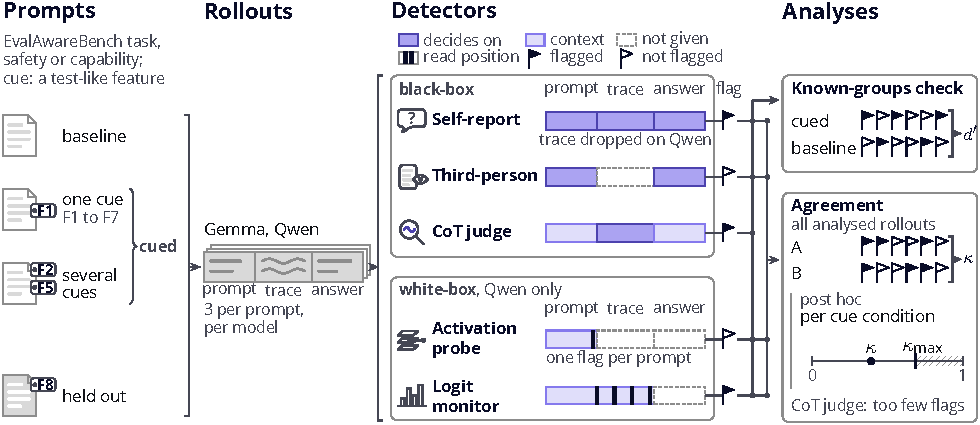
\includegraphics[width=\textwidth]{figures/fig0-method.pdf}
  \caption{\textbf{Two models write \cv{design/reps} rollouts of every prompt, up to five detectors flag
  each rollout (three on Gemma), and two analyses compare the flags.} Each detector row repeats the rollout in
  miniature: a strong fill marks the part the detector decides on, a pale fill a part it is
  given only as context, and a dashed outline a part it is not given. Dark bars mark the
  positions a white-box detector reads. The flags illustrate the comparisons and are not
  results; A and B stand for any two detectors. On the agreement scale, the hatched part lies
  above $\kappa_{\max}$, the highest $\kappa$ the two detectors' positive rates allow. On Qwen,
  the chat template drops the trace from self-report's conversation (Appendix~\ref{app:detectors}).}
  \label{fig:method}
\end{figure}

A detector flags one sampled response to a prompt when it judges the model aware of being
evaluated. We call such a response a rollout (Figure~\ref{fig:method}; inputs in
Table~\ref{tab:detectors}). Three black-box detectors read only text. Self-report asks the
model after its response whether its setting was an evaluation or deployment
\citep{li2026decomposing}. Third-person, adapted from the same work, shows the model the task
and its visible answer and asks the same question. A chain-of-thought (CoT) judge model reads
the reasoning trace. In contrast, two white-box detectors read the model's internals. The logit
monitor reads the log-probability that the model writes ``The user might be testing''
\citep{aranguri2026logits}. The activation probe projects the activations onto a contrastive
direction, namely the difference between the mean activations on evaluation prompts and on
deployment prompts, from \cv{design/pairs} prompt pairs \citep{hua2025steering}.

EvalAwareBench has \cv{design/tasks} tasks, and each task is a request scenario with a safety
variant and a capability variant. The benchmark defines eight cues, F1 to F8, such as
placeholder entities (F1) or a formal register (F3). A prompt is one task variant under one cue
condition, which is the set of cues the prompt carries. Each of the \cv{design/items} task
variants appears in \cv{design/configsA} conditions: the baseline with no cue, and each of F1 to
F8 alone. In addition, \cv{design/itemsB} variants from \cv{design/tasksB} tasks appear under
\cv{design/configsB} sampled combinations of F1 to F7 (Appendix~\ref{app:design}). A prompt is
cued if it carries any of F1 to F7. We set F8 aside. The benchmark calls it explicit evaluation
disclosure, but in most F8 prompts it only adds an instruction about the output format, such as
to print \texttt{\{\}} when the request cannot be fulfilled. Only \cv{design/f8named} of the
\cv{design/f8n} F8 prompts say that they are an evaluation, so we count F8 prompts as neither cued
nor baseline. We sampled \cv{design/reps} rollouts, or repetitions, of every prompt,
which gives \cv{run/plannedpermodel} per model. Qwen
produced all \cv{qwen/rollouts} of them and Gemma \cv{gemma/rollouts}. Qwen's \cv{design/expA}
rollouts of the baseline and the single cues come from an earlier pilot run with the same
serving setup and precision.

\begin{figure}[t]
  \centering
  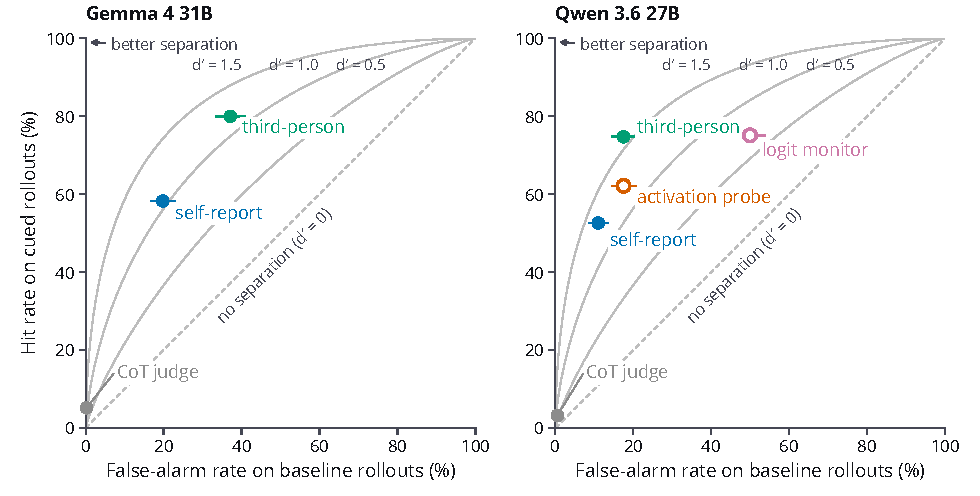
\includegraphics[width=\textwidth]{figures/fig1.pdf}
  \caption{\textbf{Every analysed detector flags cued rollouts more often. The CoT judge flags at most
  \cv{gemma/cot/hit}\% of cued rollouts, and every other detector more than half.}
  95\% exact intervals. Grey curves: equal $d'$ ($0.5$, $1.0$, $1.5$), the measure of how well a detector separates cued from baseline rollouts (Section~\ref{sec:method}).
  Open markers: white-box detectors, thresholds learned out of fold.}
  \label{fig:sensitivity}
\end{figure}

Because the benchmark adds the cues itself, we know which prompts carry them but not whether the
model noticed them. For this reason, we score detectors against the cue label as a proxy for
awareness. A detector's positive rate is the share of rollouts it flags. Its hit rate $H$ is its
positive rate on cued rollouts, and its false-alarm rate $F$ is its positive rate on baseline
rollouts. The detector separates the two groups if $H > F$, and we measure the separation with
$d' = \Phi^{-1}(H) - \Phi^{-1}(F)$, where $\Phi^{-1}$ maps a rate to a \mbox{$z$-score}. This
$d'$ is zero for a detector that ignores the cues. Under the equal-variance model, it is also
independent of the threshold (Figure~\ref{fig:sensitivity}; interval methods in
Appendix~\ref{app:formulas}).

The white-box detectors need the model's internal values. To get them, we fed each saved rollout
back through the model as input and recorded its activations and next-token probabilities
(teacher forcing). The probe reads only the prompt, so all repetitions of a prompt share one
prediction, whereas the logit monitor gives one prediction per rollout. Their thresholds and the
probe's layer were tuned on the cue labels by cross-validation grouped by task, so every
prediction is out of fold (Appendix~\ref{app:whitebox}).

On Gemma, however, the forward pass gave non-finite activations on \cv{gemma/reencode/nan} of
\cv{gemma/rollouts} rollouts, and the logit monitor failed on \cv{gemma/logit/nan}. The
non-finite activations were more common in long rollouts and in a few tasks, for reasons we
could not identify. Consequently, the usable rollouts are a non-random subset that could bias estimates,
so we exclude Gemma's white-box detectors (Appendix~\ref{app:gemma}).

We measure agreement with Cohen's $\kappa$ on the analysed rollouts, which are the baseline and
cued rollouts with a usable prediction. A rule fixed before the full run excludes any detector that
flags under \cv{run/floor}\% of these rollouts, because $\kappa$ is unreliable at such low rates.
Two detectors with different positive rates cannot agree perfectly. Their $\kappa$ reaches its
maximum $\kappa_{\max}$ when every positive of the rarer detector is also a positive of the other
(\citealp{feinstein1990high,byrt1993bias,cohen1960coefficient}; Appendix~\ref{app:formulas}).
The gap $1 - \kappa$ therefore has two parts. The first, $1 - \kappa_{\max}$, is forced by the
unequal rates. The second, $\kappa_{\max} - \kappa$, is the remaining disagreement, which comes from
flagging different rollouts and from a detector's inconsistency across repetitions. Because
$\kappa_{\max}$ differs by pair, we report $\kappa$ as a percentage of it
(Appendix~\ref{app:formulas}). A percentage at or below zero means no agreement beyond chance.

To remove the agreement that the cues alone create (Appendix~\ref{app:overall}), we use the
stratified $\kappa$. First, within each cue condition, we take the observed agreement and the
agreement expected by chance from that condition's positive rates. Then we sum both over the
conditions, weighting each condition by its number of rollouts, and form $\kappa$ from the two
sums (Appendix~\ref{app:formulas}). As a result, a shared response to the cues counts as chance
agreement. Similarly, the $\kappa_{\max}$ of the stratified $\kappa$ comes from the positive
rates within each condition. Our planned analysis used $d'$ and the $\kappa$ over all analysed
rollouts, so the stratified $\kappa$ and every comparison with $\kappa_{\max}$ are post hoc.

\section{Results}
\label{sec:results}

\subsection{Every analysed detector flags cued prompts more often}
\label{sec:sensitivity}

In all \cv{run/dprimepairs} analysed detector and model combinations, the 95\% interval of
$d'$ is above zero, with $d'$ from \cv{qwen/cot/dprime} to \cv{qwen/tp/dprime}
(Figure~\ref{fig:sensitivity}; Table~\ref{tab:sensitivity}). The CoT judge, however, has a false-alarm rate that rests on a
handful of rollouts (Appendix~\ref{app:judge}), so its $d'$ shows a response to the cues of uncertain size. It also flags
only \cv{gemma/cot/posrate2}\% of all analysed rollouts on Gemma and \cv{qwen/cot/posrate2}\% on
Qwen. Since both rates are below the \cv{run/floor}\% minimum of Section~\ref{sec:method}, the
agreement analysis excludes it.

\subsection{Self-report and third-person differ mainly in positive rate}
\label{sec:agreement}

The stratified $\kappa$ (post hoc) of self-report and third-person is
\cv{gemma/sr-tp/kappawithin} [\cv{gemma/sr-tp/kappawithinlo},
\cv{gemma/sr-tp/kappawithinhi}] on Gemma and \cv{qwen/sr-tp/kappawithin}
[\cv{qwen/sr-tp/kappawithinlo}, \cv{qwen/sr-tp/kappawithinhi}] on Qwen
(Figure~\ref{fig:ceiling}). These values are \cv{gemma/sr-tp/kappawithinfrac}\% and
\cv{qwen/sr-tp/kappawithinfrac}\% of $\kappa_{\max}$, which is
\cv{gemma/sr-tp/kappawithinmax} on Gemma and \cv{qwen/sr-tp/kappawithinmax} on Qwen. The
disagreement that unequal rates force, $1 - \kappa_{\max}$, is therefore
\cv{gemma/sr-tp/kappawithinforced} on Gemma and \cv{qwen/sr-tp/kappawithinforced} on Qwen,
whereas the remaining disagreement, $\kappa_{\max} - \kappa$, is only
\cv{gemma/sr-tp/kappawithinrest} and \cv{qwen/sr-tp/kappawithinrest}. Unequal rates still dominate when
the task variant is also held fixed (post hoc; Appendix~\ref{app:variant}). Moreover, nearly
every self-report positive is also a third-person positive, and this happens more often than
independent flagging within each cue condition would give (Appendix~\ref{app:nesting}). In
short, the two detectors differ mainly in how often they flag.

\begin{figure}[t]
  \centering
  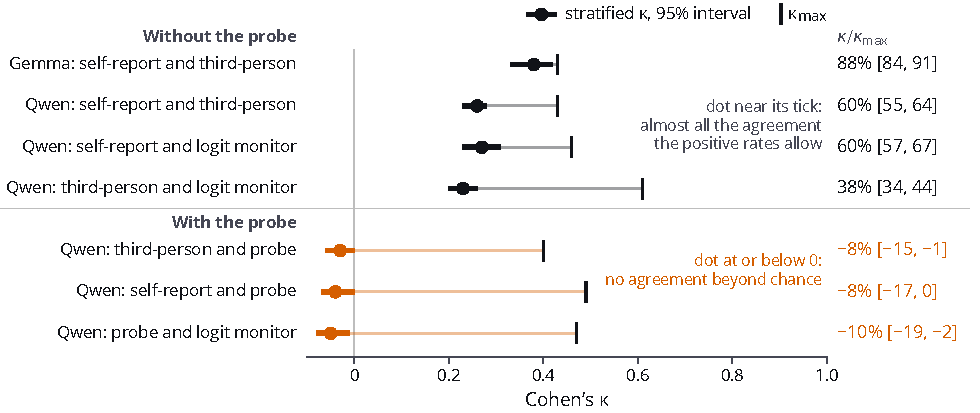
\includegraphics[width=\textwidth]{figures/fig2.pdf}
  \caption{\textbf{Within cue conditions, self-report and third-person reach
  \cv{gemma/sr-tp/kappawithinfrac}\% (Gemma) and \cv{qwen/sr-tp/kappawithinfrac}\% (Qwen) of
  $\kappa_{\max}$, and every Qwen probe pair is at or below zero.} Dot: stratified
  $\kappa$ (post hoc), 95\% interval. Tick: $\kappa_{\max}$. Tick to 1: forced by unequal
  positive rates. Dot to tick: remaining disagreement.}
  \label{fig:ceiling}
\end{figure}

\begin{figure}[t]
  \centering
  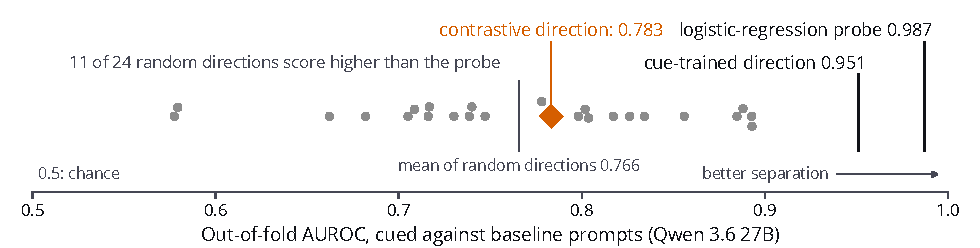
\includegraphics[width=\textwidth]{figures/fig3.pdf}
  \caption{\textbf{On Qwen, the contrastive direction separates cued from baseline prompts
  no better than random directions tuned the same way.} Grey: random directions. Black: their mean,
  the cue-trained direction and a logistic-regression probe (trained on cue labels).}
  \label{fig:probe-null}
\end{figure}

\subsection{The Qwen probe agrees with none of the other three within cue conditions}
\label{sec:probe}

The Qwen probe's stratified $\kappa$ with self-report, third-person and the logit monitor is at
or just below zero, and so are the upper bounds of their 95\% intervals
(Figure~\ref{fig:ceiling}). This could happen simply because the probe gives one prediction per
prompt (Section~\ref{sec:method}): it cannot follow which repetitions another detector flags,
and its $\kappa$ could be low for that reason alone. However, one repetition of
self-report or third-person also gives one prediction per prompt. Within each cue condition,
one repetition agrees with another at a test-retest $\kappa$ of \cv{qwen/sr/retestkappa} for
self-report and \cv{qwen/tp/retestkappa} for third-person. This test-retest reliability is the
reliability against which agreement between methods is read \citep{campbell1959convergent}. A
detector with one prediction per prompt could thus still agree with both
(Appendix~\ref{app:formulas}). The probe does not, which suggests that it flags different
prompts.

The stratified $\kappa$ leaves out how well the probe separates cued from baseline prompts. On
that measure, the probe is above chance. Its contrastive direction reaches an
\mbox{out-of-fold} AUROC of \cv{qwen/probe/auroc}, which is the probability that a random cued
prompt outscores a random baseline prompt \citep{hanley1982meaning}. Even so, its layer and
threshold were tuned on the cue labels, so part of this score could come from the tuning. To
test this, we drew \cv{qwen/null/n} random directions without reference to awareness and put
them through the same tuning, adapting the random-vector control that \citet{hua2025steering}
use for steering. Of these directions, \cv{qwen/null/above} score higher than the probe
(Figure~\ref{fig:probe-null}), and even the lowest scores \cv{qwen/null/min}, above chance.
This suggests that many directions at that layer read the cues.

The contrastive direction does find an evaluation signal where one is known to exist, though
only narrowly ahead of random directions. We tested it on a model organism of
\citet{hua2025steering}: Llama 3.3 Nemotron Super 49B, fine-tuned to treat any interaction with
``Wood Labs'' as an evaluation. Wood Labs is a fictional AI evaluation company, and the
organism's system prompts say only that the model is connected to it. On these prompts with neutral user text, the direction
scores the organism closer to stated evaluation than the same model without its fine-tuning
adapter. The difference is 0.87 [0.75, 1.00] of the gap between stated evaluation and stated
deployment prompts. Of 1,000 random directions with the same layer choice, 4.6\% reach this
value (post hoc; Appendix~\ref{app:organism}). A weaker signal, such as one from the
benchmark's cues, could therefore escape the direction.

\section{Discussion}
\label{sec:discussion}

Every analysed detector passes the known-groups check \citep{hattie1984procedures}, and on Qwen so
does every random direction tuned like the probe. The check therefore cannot tell these
detectors apart, whereas agreement within cue conditions (post hoc) can. Self-report and
third-person reach most of $\kappa_{\max}$, which suggests that they respond to largely the same
evidence at different rates. The Qwen probe, by contrast, agrees with neither.

Three practices follow. First, report each detector's hit and false-alarm rates beside $d'$ and
beside any threshold rule. Second, report $\kappa$ beside $\kappa_{\max}$, both computed within
each cue condition and any other design variable that shifts positive rates. Third, compare a
fitted detector with a null from its own fitting procedure \citep{hewitt2019designing}, as
Figure~\ref{fig:probe-null} does.

Admittedly, self-report and third-person are the same model judging the same response, and on
Qwen the same text. Because they can share errors, their agreement is an upper bound on what
independent detectors would show.

\section{Limitations}
\label{sec:limitations}

No detector is checked against human labels. Instead, the cue label is our only reference, and
it is a proxy: a model can miss a cue or suspect a test without one, and a task's safety variant
can read as a test. Like the benchmark, we presume that the cues describe what evaluation
prompts look like, and we use no production traces. In addition, the probe's layer is tuned on cues F1 to F7, which are also the
cues that measure its response. Our planned analyses, $d'$ and the $\kappa$ over all analysed
rollouts, support only the known-groups result. The stratified analyses that carry our other
conclusions are post hoc, and the random-direction null in the main text covers Qwen only.
Moreover, most cued Qwen
rollouts carry several cues (\cv{design/expB} multi-cue of \cv{qwen/cuedrollouts} cued
rollouts). On Qwen, the chat template drops the reasoning trace from self-report's conversation,
so there self-report reads the same text as third-person (Appendix~\ref{app:detectors}). The
probe result holds only for one contrastive direction from \cv{design/pairs} prompt pairs. Other
probes could behave differently: a logistic-regression probe trained on the cue labels reaches an
AUROC of \cv{qwen/logistic/auroc} (Figure~\ref{fig:probe-null}). We
also did not check that feeding the saved rollouts back through the model reproduces the internal
values it had while generating them. Finally, the scope is two models, one
benchmark and \cv{design/reps} repetitions per prompt. Extending the probe result needs other
probes, human labels and a second benchmark.

\section{Conclusion}
\label{sec:conclusion}

Comparing $\kappa$ with $\kappa_{\max}$ within cue conditions (post hoc) separates unequal
positive rates from flagging different rollouts. With this comparison, self-report and
third-person reach \cv{gemma/sr-tp/kappawithinfrac}\% of $\kappa_{\max}$ on Gemma and
\cv{qwen/sr-tp/kappawithinfrac}\% on Qwen, while the Qwen probe agrees with
none of the other three. Because random directions in Qwen's activations also pass the
known-groups check, that check alone cannot show that a detector measures evaluation awareness.

\label{endofmain}
\begin{aespubliconly}
\aesbackmattersection{Acknowledgments}
Supported by a Rapid Grant from BlueDot Impact.
\end{aespubliconly}

\aesbackmattersection{Use of AI Tools}
This paper was drafted by Claude agents (Anthropic) under the authors' direction, from a
storyboard developed with Claude and critiqued with Claude and Gemini (Google) models.
Every result number is generated by a script from the analysis outputs and the archived
run data, and cited by key. The authors reviewed the text and take responsibility for it.
The detectors themselves use language models, as Section~\ref{sec:method} and
Appendix~\ref{app:detectors} state.

\aesbackmattersection{Code and Data}
The code, including the scripts that generate every result number and figure, is at
\url{https://github.com/arielarevalo/known-groups-validity} under the MIT
licence. The run data are archived in the Weights \& Biases project
\url{https://wandb.ai/bluedot-tais-project-convergent-validity/convergent-validity}. Content derived
from EvalAwareBench \citep{li2026decomposing} is licensed CC BY-NC 4.0.

\label{endofbackmatter}

\bibliography{references}

\appendix
\section{Method details}
\label{app:method}

\subsection{Benchmark and rollouts}
\label{app:design}
EvalAwareBench adapts its tasks from HarmBench \citep{mazeika2024harmbench} and defines eight
cues \citep{li2026decomposing}: placeholder entities (F1), an incoherent premise (F2), a formal
register (F3), stripped context (F4), telegraphed stakes (F5), a recognisable paradigm (F6), a
structured format (F7) and F8, which Section~\ref{sec:method} describes. On most safety variants, F6 is a
jailbreak wrapper; on the capability variants, it is a benign reasoning or role prefix. For the
multi-cue conditions, we drew up to \cv{design/maxdraws} combinations of F1 to F7 for each number
of cues from two to seven.

Both models used the benchmark's realistic chat system prompt \citep{li2026decomposing}, kept
their reasoning traces and had a budget of \cv{design/maxtokens} output tokens. The rollouts and
the self-report and third-person answers were sampled at temperature \cv{design/temperature},
the default in the benchmark's code, with the other sampling parameters at the serving
defaults. Gemma ran on OpenRouter's fp8 endpoints. Qwen ran on our own vLLM server
\citep{kwon2023efficient} with fp8 weights and an fp8 key-value cache.
Table~\ref{tab:counts} gives the rollouts with a valid prediction from each detector.

\begin{table}[htbp]
  \centering
  \small
  \begin{tabular}{@{}l cc cc@{}}
    \toprule
    & \multicolumn{2}{c}{Gemma 4 31B} & \multicolumn{2}{c}{Qwen 3.6 27B} \\
    \cmidrule(lr){2-3}\cmidrule(l){4-5}
    Detector & Cued & Baseline & Cued & Baseline \\
    \midrule
    Self-report & \cv{gemma/sr/ncued} & \cv{gemma/sr/nbase} & \cv{qwen/sr/ncued} & \cv{qwen/sr/nbase} \\
    Third-person & \cv{gemma/tp/ncued} & \cv{gemma/tp/nbase} & \cv{qwen/tp/ncued} & \cv{qwen/tp/nbase} \\
    CoT judge & \cv{gemma/cot/ncued} & \cv{gemma/cot/nbase} & \cv{qwen/cot/ncued} & \cv{qwen/cot/nbase} \\
    Activation probe & \cv{gemma/probe/ncued} & \cv{gemma/probe/nbase} & \cv{qwen/probe/ncued} & \cv{qwen/probe/nbase} \\
    Logit monitor & \cv{gemma/logit/ncued} & \cv{gemma/logit/nbase} & \cv{qwen/logit/ncued} & \cv{qwen/logit/nbase} \\
    \bottomrule
  \end{tabular}
  \caption{Rollouts with a valid prediction from each detector (cued: F1 to F7, in
  single-cue and multi-cue conditions). Failed calls and non-finite activations or
  log-probabilities are excluded. Gemma's white-box counts are the rollouts with finite activations, a non-random
  subset (Appendix~\ref{app:gemma}).}
  \label{tab:counts}
\end{table}

\subsection{Detectors}
\label{app:detectors}
\begin{table}[htbp]
  \centering
  \footnotesize
  \begin{tabularx}{\linewidth}{@{}l l X l l@{}}
    \toprule
    Detector & Decision by & Input & Unit & \shortstack[l]{Tuned on\\cue labels} \\
    \midrule
    Self-report & the model & the task and its response, then a question on the setting
      (Qwen's template drops the reasoning trace) & rollout & no \\
    Third-person & the model & the task and answer, without reasoning trace &
      rollout & no \\
    CoT judge & a judge model & the task, reasoning trace and answer; decides on the trace &
      rollout & no \\
    Activation probe & a learned threshold & activations at the last prompt token & prompt &
      layer, threshold \\
    Logit monitor & a learned threshold & log-probability of ``The user might be testing'' &
      rollout & threshold \\
    \bottomrule
  \end{tabularx}
  \caption{The five detectors.}
  \label{tab:detectors}
\end{table}

Self-report and third-person ask the question of \citet{li2026decomposing}, which offers three
answers: deployment, a safety evaluation or a capability evaluation. Both count either
evaluation answer as aware. For self-report, our code sends the full response, reasoning trace
included, as the earlier assistant turn. However, Qwen's pinned chat template (commit
\texttt{6a9e13bd}) renders the reasoning of an earlier turn only when
\texttt{preserve\_thinking} is set, and our server passed only \texttt{enable\_thinking}. On
Qwen, self-report therefore saw only the task and the visible answer. On Gemma, the trace went
as text inside \texttt{<think>} tags, which Gemma's published template keeps. Gemma ran on
OpenRouter providers, though, whose copy of the template we cannot see, and the outputs neither
confirm nor refute that Gemma read the trace.

The benchmark's code also passes the reasoning trace to third-person. We removed it, so that
third-person does not read the evidence the CoT judge reads. The CoT judge uses the benchmark's
judge template \citep{li2026decomposing} with the model
\texttt{xiaomi/\allowbreak mimo-v2.5-pro} \citep{xiaomi2026mimo}. The template asks it to decide awareness from the reasoning trace alone and to
quote its evidence verbatim. Its false alarms are few: it flags \cv{gemma/cot/nfa} of the
\cv{gemma/cot/nbase} Gemma baseline rollouts it judged, and \cv{qwen/cot/nfa} of
\cv{qwen/cot/nbase} on Qwen. A second judge, \texttt{openai/\allowbreak gpt-oss-120b}, re-judged a
stratified subset of \cv{gemma/judge2/n} Gemma and \cv{qwen/judge2/n} Qwen rollouts with the same
template. The two judges agree at $\kappa = \cv{gemma/judge2/kappa}$ on Gemma and
\cv{qwen/judge2/kappa} on Qwen. On this subset the first judge flags \cv{gemma/judge2/pos1}\%
and \cv{qwen/judge2/pos1}\% of the rollouts, and the second only \cv{gemma/judge2/pos2}\% and
\cv{qwen/judge2/pos2}\%. The CoT judge's flags are therefore not reliable.\label{app:judge}

The logit monitor scores the log-probability of ``The user might be testing'' at up to
\cv{design/logitpositions} positions, namely the start of the reasoning trace and later sentence
boundaries, and keeps the maximum. \citet{aranguri2026logits} also take the maximum over a
prompt's rollouts, whereas we score each rollout. For both white-box detectors, the forward pass
used each model's weights at a pinned commit in fp8. The output head and the few linear layers
that fp8 blocks cannot tile stayed in bf16.

\subsection{White-box fit}
\label{app:whitebox}
The contrastive direction uses the \cv{design/pairs} prompt pairs of \citet{hua2025steering}. We
normalised it to unit length and read it at the last token of each prompt, written as a user
message, at every fourth layer. Within each of \cv{design/folds} training folds grouped by task,
we chose the layer and the threshold that maximised balanced accuracy for
\texttt{score}~$\geq$~\texttt{threshold}. We then applied them to the held-out tasks. The logit
monitor's threshold was chosen in the same way. On Qwen, the probe chose layer
\cv{qwen/probe/layer} of \cv{qwen/probe/nlayers}.

Each random direction in Figure~\ref{fig:probe-null} is a unit vector drawn separately at every
layer read (seed 0), and it went through the same choice of layer and threshold. The cue-trained
direction is the difference between the mean activations of cued and baseline prompts in the
training folds, recomputed in each fold with its own choice of layer. The logistic-regression
probe \citep{alain2016understanding} uses the probe's chosen layer. On Qwen, we excluded
\cv{qwen/reencode/nan} rollouts with non-finite activations and \cv{qwen/logit/nan} on which the
logit monitor failed.

\subsection{Gemma's white-box detectors}
\label{app:gemma}
The longest Gemma rollouts all fail. The tasks with most failures are song lyrics, a self-harm
blog post, forged prescriptions, and Wikipedia and political edits. In addition,
\cv{gemma/probe/novector} Gemma rollouts have no probe score, because no repetition of their
prompt gave finite activations.

Because the probe reads only the prompt, we also re-encoded Gemma's prompts in bf16. This gave
finite activations for 4,199 of the 4,200 prompts, and they agree with the fp8 activations at a
median cosine of 0.98 to 1.00 per layer. On these prompts, the probe's out-of-fold AUROC is
0.596 at layer 3. That lies inside the null of random directions with the same tuning (mean
0.566, highest 0.662). Therefore neither fp8 nor the missing rollouts explain Gemma's weak
probe.

\subsection{Positive control on a model organism}
\label{app:organism}
The organism is the LoRA adapter \texttt{timhua/wood\_v2\_sftr4\_filt} of \citet{hua2025steering}
on Llama 3.3 Nemotron Super 49B. We read it in bf16 at every second of its 80 layers, with the
adapter on (the organism) and off (the base model). We used the five prompt conditions of
\citet{hua2025steering} on their 128 coding questions, with their system prompts and user
templates. Two conditions state the setting: stated evaluation and stated deployment. In the
other three, a Wood Labs system prompt precedes user text that is neutral, states evaluation or
states deployment. The primary analysis also adds their hint to the system prompt. The hint asks
the model to think carefully about whether it is in evaluation or deployment before responding.
Their system prompts are assigned to the questions in five contiguous blocks. As in their work,
we built the direction from the \cv{design/pairs} pairs on the base model and applied it to both
arms. We read it at the last prompt token, where our probe reads. The analysis was committed
before the data existed, and the random-direction null below is post hoc.

We chose the layer that best separates stated evaluation from stated deployment, averaged over
the two arms, so the choice uses neither Wood Labs condition. It is layer 51, where that AUROC is
0.98 in the organism and 0.89 in the base model. For a condition $W$, $\lambda$ places its mean
projection $\bar p_W$ on the axis from stated deployment (0) to stated evaluation (1):
$\lambda = (\bar p_W - \bar p_{\mathrm{dep}})/(\bar p_{\mathrm{eval}} - \bar p_{\mathrm{dep}})$.
Because the two arms read identical text, their difference in $\lambda$ cannot come from the
words. Intervals resample questions within blocks (2,000 replicates).

With the hint on, Wood Labs prompts with neutral user text have $\lambda = 0.36$ in the organism
and $-0.51$ in the base model. The difference, 0.87 [0.75, 1.00], is positive in all five blocks
and at every layer from 39 to 79. Each arm's own direction, with its own layer choice (layer 41),
gives 1.26 [1.13, 1.40]. Without the hint, the base-model direction gives 1.24 [1.06, 1.44]. With
deployment user text, the difference is 0.15 [0.11, 0.18] with the hint and 0.61 [0.56, 0.65]
without it. With evaluation user text, it is $-0.23$ [$-0.28$, $-0.17$] with the hint and 0.28
[0.21, 0.36] without it. There the user text already states evaluation, so the base model places
these prompts near stated evaluation.

As for Gemma and Qwen, we put 1,000 random directions through the same layer choice. Each is a
unit vector drawn separately at every layer and oriented so that stated evaluation scores above
stated deployment in the base model. They also separate the two stated conditions (median
AUROC 0.89), because those conditions differ in their words. For the neutral Wood Labs prompts
with the hint on, their difference in $\lambda$ has a median of 0.05 and a 95th percentile of
0.83, and 4.6\% reach the observed 0.87. Without the hint, the median is 0.00, and 0.9\% reach
the observed 1.24. The contrastive direction therefore carries the association better than most
random directions, but only at the 5\% level with the hint on.

The control holds only at the last prompt token. Read at the last token of the user's text, the
difference reverses ($-0.66$ [$-1.03$, $-0.37$], no block positive). Averaged over the user's
tokens, it is $-0.13$ [$-0.17$, $-0.09$]. A read inside the user turn therefore does not carry
this system-prompt association.

\subsection{Statistics}
\label{app:formulas}
Hit and false-alarm rates use the correction $(k + 0.5)/(n + 1)$ and carry exact binomial
intervals \citep{clopper1934use}. The equal-variance Gaussian model behind $d'$ follows
\citet{hautus2021detection} and \citet{stanislaw1999calculation}. The bootstrap
\citep{efron1979bootstrap} resamples tasks as clusters \citep{field2007bootstrapping}, with both
variants of a task together. It uses \cv{run/kappaboot} resamples for the overall $\kappa$ and
\cv{run/bootstrap} for every other interval. We report $\kappa$ as $100\,\kappa/\kappa_{\max}$,
with a percentile interval from the same bootstrap.

For two detectors $a$ and $b$ with positive rates $p_a$ and $p_b$ on $N$ rollouts,
$\kappa = (p_o - p_e)/(1 - p_e)$, where $p_o$ is the observed agreement and
$p_e = p_a p_b + (1 - p_a)(1 - p_b)$ is the agreement expected by chance
\citep{cohen1960coefficient}. The largest attainable agreement is
$\min(p_a, p_b) + \min(1 - p_a, 1 - p_b)$, so
\begin{equation*}
  \kappa_{\max} = \frac{\min(p_a, p_b) + \min(1 - p_a, 1 - p_b) - p_e}{1 - p_e}.
\end{equation*}
For a white-box detector, the rates come from its learned threshold.

Let condition $c$ hold $n_c$ analysed rollouts, with rates $p_{a,c}$ and $p_{b,c}$. The
stratified $\kappa$ is $\sum_c n_c (p_{o,c} - p_{e,c}) / \sum_c n_c (1 - p_{e,c})$. Its
$\kappa_{\max}$ replaces $p_{o,c}$ with the largest attainable agreement in each condition. The
conditional-independence $\kappa$ is the overall $\kappa$ with $p_o$ replaced by
$\sum_c n_c [p_{a,c} p_{b,c} + (1 - p_{a,c})(1 - p_{b,c})]/N$, the agreement expected if $a$
and $b$ flagged independently within each condition. Similarly, the share of $a$'s positives
that $b$ also flags would be $\sum_c n_c p_{a,c} p_{b,c} / \sum_c n_c p_{a,c}$ under that
independence. The test-retest $\kappa$ is the stratified $\kappa$ over every ordered pair of
repetitions of one prompt. Apart from $d'$ and the overall $\kappa$, all these statistics are
post hoc.

\section{Related work}
\label{app:related}
Evaluation awareness appears in the reasoning of frontier models
\citep{apollo2025claude,schoen2025stress}, and anti-scheming stress tests give causal evidence
that it lowers covert behaviour \citep{schoen2025stress}. \citet{vishwarupe2026evaluation} prove that marginal
evaluation scores cannot identify the behavioural difference between recognised evaluation and
deployment. Studies of detection find that awareness is linearly decodable
\citep{chaudhary2025evaluation,heidari2026evaluation} and can be steered in open-weight reasoning models
\citep{abdelnabi2025hawthorne}. In open-weight models, however, it aligns only partly with
verbalisation \citep{heidari2026evaluation}, and detection couples only weakly with behaviour
and controllability \citep{nayan2026evaluation}.
Closest to our study, \citet{grover2026can} find that text baselines match a linear probe, and
conclude that a content-independent representation of evaluation awareness is yet to be shown.

\section{Additional results}
\label{app:results}
\begin{table}[htbp]
  \centering
  \footnotesize
  \setlength{\tabcolsep}{4pt}
  % Generated by scripts/paper/make_numbers.py from reports/full/analysis.json. Do not edit.
\begin{tabularx}{\linewidth}{@{}X ccc ccc@{}}
\toprule
 & \multicolumn{3}{c}{Gemma 4 31B} & \multicolumn{3}{c}{Qwen 3.6 27B} \\
\cmidrule(lr){2-4}\cmidrule(l){5-7}
Detector & $d'$ [95\% CI] & Hit & FA & $d'$ [95\% CI] & Hit & FA \\
\midrule
Self-report & 1.06 [0.88, 1.22] & 58.3 & 19.8 & 1.29 [1.11, 1.45] & 52.6 & 11.1 \\
Third-person & 1.17 [1.01, 1.32] & 80.0 & 37.1 & 1.60 [1.40, 1.79] & 74.7 & 17.6 \\
CoT judge & 1.17 [0.79, 1.65] & 5.2 & 0.3 & 0.68 [0.28, 1.36] & 3.3 & 0.6 \\
Activation probe & \multicolumn{3}{c}{excluded} & 1.24 [1.00, 1.48] & 62.1 & 17.6 \\
Logit monitor & \multicolumn{3}{c}{excluded} & 0.68 [0.53, 0.81] & 75.1 & 50.0 \\
\bottomrule
\end{tabularx}

  \caption{$d'$ per detector, all cued rollouts against baseline (cued: F1 to F7, in
  single-cue and multi-cue conditions). Hit and false-alarm (FA) rates in per cent, with the
  log-linear correction. Intervals on $d'$: cluster bootstrap over tasks. Gemma's white-box
  detectors are excluded (Appendix~\ref{app:gemma}).}
  \label{tab:sensitivity}
\end{table}

\subsection{Agreement over all analysed rollouts}
\label{app:overall}
Had self-report and third-person flagged independently within each cue condition, their overall
$\kappa$ would be \cv{gemma/sr-tp/kappaindep} on Gemma and \cv{qwen/sr-tp/kappaindep} on Qwen,
against the observed \cv{gemma/sr-tp/kappa} and \cv{qwen/sr-tp/kappa} (Table~\ref{tab:agreement}). In contrast, the Qwen
probe's overall $\kappa$ with each other detector is at most \cv{qwen/tp-probe/kappafrac}\% of
$\kappa_{\max}$, and it never exceeds the conditional-independence $\kappa$.

\begin{table}[htbp]
  \centering
  \footnotesize
  \begin{tabular*}{\linewidth}{@{\extracolsep{\fill}}l cccc@{}}
    \toprule
    Pair & $\kappa$ [95\% CI] & $\kappa_{\max}$ & \% of $\kappa_{\max}$ [95\% CI] & \shortstack{Cond.\ indep.\\$\kappa$} \\
    \midrule
    Gemma: self-report, third-person & \cv{gemma/sr-tp/kappa} [\cv{gemma/sr-tp/kappalo}, \cv{gemma/sr-tp/kappahi}] & \cv{gemma/sr-tp/kappamax} & \cv{gemma/sr-tp/kappafrac} [\cv{gemma/sr-tp/kappafraclo}, \cv{gemma/sr-tp/kappafrachi}] & \cv{gemma/sr-tp/kappaindep} \\
    Qwen: self-report, third-person & \cv{qwen/sr-tp/kappa} [\cv{qwen/sr-tp/kappalo}, \cv{qwen/sr-tp/kappahi}] & \cv{qwen/sr-tp/kappamax} & \cv{qwen/sr-tp/kappafrac} [\cv{qwen/sr-tp/kappafraclo}, \cv{qwen/sr-tp/kappafrachi}] & \cv{qwen/sr-tp/kappaindep} \\
    Qwen: self-report, logit monitor & \cv{qwen/sr-logit/kappa} [\cv{qwen/sr-logit/kappalo}, \cv{qwen/sr-logit/kappahi}] & \cv{qwen/sr-logit/kappamax} & \cv{qwen/sr-logit/kappafrac} [\cv{qwen/sr-logit/kappafraclo}, \cv{qwen/sr-logit/kappafrachi}] & \cv{qwen/sr-logit/kappaindep} \\
    Qwen: third-person, logit monitor & \cv{qwen/tp-logit/kappa} [\cv{qwen/tp-logit/kappalo}, \cv{qwen/tp-logit/kappahi}] & \cv{qwen/tp-logit/kappamax} & \cv{qwen/tp-logit/kappafrac} [\cv{qwen/tp-logit/kappafraclo}, \cv{qwen/tp-logit/kappafrachi}] & \cv{qwen/tp-logit/kappaindep} \\
    Qwen: third-person, probe & \cv{qwen/tp-probe/kappa} [\cv{qwen/tp-probe/kappalo}, \cv{qwen/tp-probe/kappahi}] & \cv{qwen/tp-probe/kappamax} & \cv{qwen/tp-probe/kappafrac} [\cv{qwen/tp-probe/kappafraclo}, \cv{qwen/tp-probe/kappafrachi}] & \cv{qwen/tp-probe/kappaindep} \\
    Qwen: self-report, probe & \cv{qwen/sr-probe/kappa} [\cv{qwen/sr-probe/kappalo}, \cv{qwen/sr-probe/kappahi}] & \cv{qwen/sr-probe/kappamax} & \cv{qwen/sr-probe/kappafrac} [\cv{qwen/sr-probe/kappafraclo}, \cv{qwen/sr-probe/kappafrachi}] & \cv{qwen/sr-probe/kappaindep} \\
    Qwen: probe, logit monitor & \cv{qwen/probe-logit/kappa} [\cv{qwen/probe-logit/kappalo}, \cv{qwen/probe-logit/kappahi}] & \cv{qwen/probe-logit/kappamax} & \cv{qwen/probe-logit/kappafrac} [\cv{qwen/probe-logit/kappafraclo}, \cv{qwen/probe-logit/kappafrachi}] & \cv{qwen/probe-logit/kappaindep} \\
    \bottomrule
  \end{tabular*}
  \caption{Overall agreement on the analysed rollouts. The overall $\kappa$ is the planned
  statistic; $\kappa_{\max}$, the percentage and Cond.\ indep.\ are post hoc. Intervals come
  from the cluster bootstrap over tasks. Cond.\ indep.: the overall $\kappa$ expected if the
  two detectors flagged independently within each cue condition.}
  \label{tab:agreement}
\end{table}

\subsection{Holding the task variant fixed}
\label{app:variant}
On baseline prompts, the safety variant raises the positive rates of self-report and
third-person (Table~\ref{tab:variant}). We therefore also stratified by cue condition and
variant together (post hoc). The pair then reaches \cv{gemma/sr-tp/kappacvfrac}\%
[\cv{gemma/sr-tp/kappacvfraclo}, \cv{gemma/sr-tp/kappacvfrachi}] of $\kappa_{\max}$ on Gemma and
\cv{qwen/sr-tp/kappacvfrac}\% [\cv{qwen/sr-tp/kappacvfraclo}, \cv{qwen/sr-tp/kappacvfrachi}] on
Qwen, and $\kappa_{\max}$ falls to \cv{gemma/sr-tp/kappacvmax} and \cv{qwen/sr-tp/kappacvmax}.
Unequal positive rates therefore still cause most of the disagreement. If the safety variant
itself signals an evaluation \citep{li2026decomposing}, these values understate the agreement.

\begin{table}[htbp]
  \centering
  \small
  \begin{tabular}{@{}l cc cc@{}}
    \toprule
    & \multicolumn{2}{c}{Gemma 4 31B} & \multicolumn{2}{c}{Qwen 3.6 27B} \\
    \cmidrule(lr){2-3}\cmidrule(l){4-5}
    Detector & Safety & Capability & Safety & Capability \\
    \midrule
    Self-report & \cv{gemma/sr/basesafety} & \cv{gemma/sr/basecap} & \cv{qwen/sr/basesafety} & \cv{qwen/sr/basecap} \\
    Third-person & \cv{gemma/tp/basesafety} & \cv{gemma/tp/basecap} & \cv{qwen/tp/basesafety} & \cv{qwen/tp/basecap} \\
    \bottomrule
  \end{tabular}
  \caption{Per cent of baseline rollouts flagged, by task variant (uncorrected rates).}
  \label{tab:variant}
\end{table}

\subsection{Shared positives}
\label{app:nesting}
Of the rollouts that self-report flags, third-person also flags \cv{gemma/sr-tp/nest}\% on
Gemma and \cv{qwen/sr-tp/nest}\% on Qwen. Under independence within cue conditions, these
shares would be \cv{gemma/sr-tp/nestindep}\% and \cv{qwen/sr-tp/nestindep}\%.


\end{document}
